\documentclass[11pt]{hyu_thesis}
\usepackage{tabularx}
\begin{comment}
\usepackage{tikz}
\usepgfplotslibrary{external} % creates a tight self-contained pdf figure for each tikzpicture
\tikzexternalize % comment out to debug if latex errors: generates the external pdf
\tikzset{external/force remake} % otherwise will use external pdf if it exists
\tikzset{png export/.style={
		external/system call={
			pdflatex \tikzexternalcheckshellescape
			-halt-on-error -interaction=batchmode -jobname "\image" "\texsource";
			convert -units pixelsperinch -density 600 "\image.pdf" "\image.png";
}}}
\tikzset{png export}
\tikzsetexternalprefix{tikz/} % output the pdf to an existing directory (needs to exist)
\end{comment}
\begin{document}

\abovedisplayskip=16pt
\abovedisplayshortskip=11pt
\belowdisplayskip=16pt
\belowdisplayshortskip=11pt

\newgeometry{left=0mm, right=0mm, top=20mm, bottom=20mm, head=0mm, foot=0mm}
\begin{titlepage}
	\centering
	\begin{tabularx}{185mm}{>{\centering\arraybackslash}X}
		\\[2.5cm]
		\largefont{Thesis for the degree of Doctor of Philosophy}\\[3cm]
		\fontsize{20}{12}\selectfont{Concurrent Probabilistic Tube Rearrangement Algorithm for Online Video Synopsis}
	\end{tabularx}
	\vfill
	\begin{tabularx}{185mm}{>{\centering\arraybackslash}X}
		\largefont{Moonsoo Ra}\\[3.5cm]
		\largefont{Graduate School of Hanyang University}\\[2.5cm]
		\largefont{August 2019}\\[2.5cm]
	\end{tabularx}
\end{titlepage}

\begin{titlepage}
	\centering
	\begin{tabularx}{185mm}{>{\centering\arraybackslash}X}
		\\[2cm]
		\largefont{Thesis for the degree of Doctor of Philosophy}\\[2cm]
		\fontsize{20}{12}\selectfont{Concurrent Probabilistic Tube Rearrangement Algorithm for Online Video Synopsis}
	\end{tabularx}
	\vfill
	\begin{tabularx}{185mm}{>{\centering\arraybackslash}X}
		\largefont{Thesis supervisor: Whoi-Yul Kim}\\[1.5cm]
		\largefont{A Thesis submitted to the graduate school of}\\
		\largefont{Hanyang University in partial fulfillment of the requirements}\\
		\largefont{for the degree of Doctor of Philosophy}\\[3cm]
		\largefont{Moonsoo Ra}\\[1cm]
		\largefont{August 2019}\\[1cm]
		\largefont{Department of Electronics and Computer Engineering}\\
		\largefont{Graduate School of Hanyang University}\\[1.5cm]
	\end{tabularx}
\end{titlepage}

\restoregeometry
\frontmatter

\tableofcontents
\newpage
\listoffigures
\newpage
\listoftables
\newpage

\mainmatter

\chapter*{ABSTRACT}
\addcontentsline{toc}{chapter}{\textbf{ABSTRACT}}
Video synopsis allows us to analyze security videos efficiently by condensing or shortening a long video into a short one. To generate a condensed video, moving objects are extracted in the form of object tubes. Then, these tubes are rearranged in the temporal domain using a predefined objective function. It consists of several energy terms which play important roles in making a visually appealing condensed video. Among them, collision energy creates a bottleneck in the computation because it requires two object tubes as input arguments. Existing approaches try to reduce the computation time of the collision energy calculation by reducing the number of tubes processed at once. However, those approaches are not sufficient to generate condensed video when the number of object tubes becomes large.

This dissertation presents a concurrent probabilistic tube rearrangement algorithm with fast Fourier transform (FFT) targeted for online video synopsis. Instead of representing locations of object tubes as bounding boxes, the proposed algorithm utilizes the occupation matrices, foreground masks having low resolution. Then, the collision energy can be computed by series of element-wise multiplications between the occupation matrices. In addition, this process can be accelerated by utilizing FFT and parallel processing.

To evaluate and analyze the performance of the proposed algorithm, total 10 hours long videos are captured at four different places of Hanyang University, Seoul Korea. For all the test sequences, the proposed algorithm can produce condensed videos within 0.75 seconds in average, and it is at least 6 times faster results than the existing algorithms. Moreover, resulting synopsis videos of the proposed algorithm have less collisions than its competitors. For better understanding of the proposed algorithm, effectiveness of two speed up techniques has been analyzed through the ablation study, and parameter analysis of the proposed algorithm has been conducted extensively.
\newpage

\chapter{Introduction}
\label{sec:intro}
\section{Motivation}
\label{sec:intro:motivation}
The field of security video summarization has been studied for decades to reduce burdens of browsing large amount of video footages. Earlier approaches~\cite{Smith1997,Petrovic2005,Hoferlin2011} prior to video synopsis~\cite{Rav-Acha2006,Pritch2007,Pritch2008} suffered from several disadvantages including low frame condensation ratio (FR) or missing information, when the frame length of the input video was long. Fundamental building blocks of such approaches were image frames, which means that they tried to select a subset of image frames representing the original video best. On the other hand, building blocks of video synopsis~\cite{Rav-Acha2006,Pritch2007,Pritch2008} are moving objects extracted from the scene, called \textit{object tubes}. In the video synopsis framework, the object tubes are rearranged in the temporal domain and stitched back with background images to generate a short and condensed video. This difference allows video synopsis to efficiently utilize the spatial domain of the video and to drastically improve the FR as compared to the earlier approaches.

Among the diverse research topics in video synopsis, solving the optimization problem for determining starting positions (starting labels) of the object tubes in the temporal domain greatly affects the system performance regarding computation time. This problem is simply denoted as \textit{a tube rearrangement problem}.

In the pioneering work of video synopsis by Pritch~\etal~\cite{Pritch2008}, the tube rearrangement problem is formulated as Markov Random Fields (MRFs)~\cite{Kolmogorov2004} with four energy terms: activity, collision, temporal consistency, and background consistency. The starting label for each object tube is then determined by minimizing the energy function of MRFs with a simulated annealing~\cite{Kirkpatrick1983} or greedy optimization algorithm~\cite{Cormen2009}. During the optimization process, calculating pairwise energy terms (in this case, collision and temporal consistency) becomes a bottleneck for computation speed, because such calculation has $O(TK^2)$ complexity, where $T$ is the number of time steps and $K$ is the total number of object tubes.

In order to cope with the problem, Pritch~\etal~\cite{Pritch2009} suggest
a clustering based optimization algorithm. It divides object tubes into several subsets; then, the optimization algorithm is conducted on each subset. Since the number of object tubes belonging to each subset is much smaller than $K$, execution time of the optimization algorithm is greatly reduced. However, its condensation result depends on the performance of the clustering algorithm which has a chance to
generate inappropriate clusters.

An alternative approach to tube rearrangement is an online video synopsis~\cite{Huang2014,Feng2012,Zhu2015,He2017,Fu2014}, which solves a stepwise optimization problem. In stepwise optimization, instead of considering entire object tubes at the same time, the starting labels of the object tubes are determined one by one. Therefore, it requires less computational power and memory space than batch or offline video synopsis. In addition, since online video synopsis optimizes the object tubes in chronological order, it is inessential to consider temporal and background consistencies. Therefore, the most of online video synopsis frameworks mainly consider the collision energy during the optimization.

Based on such advantages, recent studies of online video synopsis focused on finding efficient ways of solving a stepwise optimization problem: for example, the maximum a posteriori estimation~\cite{Huang2014}, a Tetris-like tube rearrangement strategy~\cite{Feng2012,Zhu2015}, and a potential collision graph~\cite{He2017}. 
Even though these existing algorithms have their own virtue, they have lack of considerations of multi-core environment, which means that there are still rooms for improvements.

In this dissertation, the tube rearrangement problem is reformulated as a suitable form for parallel processing, and the novel concurrent optimization algorithm based on 1D convolutions is proposed to accelerate the optimization process. As in other online tube rearrangement algorithms~\cite{Huang2014,Feng2012,Zhu2015,He2017,Fu2014}, the collision energy is primarily considered during the tube rearrangement. As a preprocessing step, the proposed algorithm reshapes object tubes into probabilistic occupation matrices of $\mathcal{M} \times \mathcal{N} \times \mathcal{T}$ dimension, where $\mathcal{M}$ and $\mathcal{N}$ represent the spatial domain, and $\mathcal{T}$ represents the time domain. This occupation matrix becomes a fundamental building block of the proposed algorithm. Then, the collision energy between two object tubes can be computed as element-wise multiplications of two occupation matrices. This process can be accelerated by utilizing fast Fourier transform (FFT)~\cite{Oppenheim2009} in conjunction with parallel computing; therefore, the proposed algorithm can effectively determine the starting labels of numerous object tubes in very short amount of time.

\section{Related works}
\label{sec:intro:related}
After the very first appearance of the video synopsis technique~\cite{Rav-Acha2006}, it has been improved in many different aspects. In this dissertation, recent advances in video synopsis are discussed. Especially, details of the online video synopsis framework are presented.

\begin{figure}
	\centering
	\subfloat[]
	{
		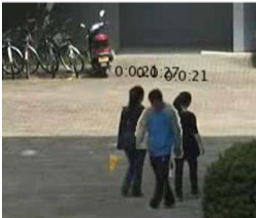
\includegraphics[width=0.2\linewidth]{ext-li01.png}
	}
	\subfloat[]
	{
		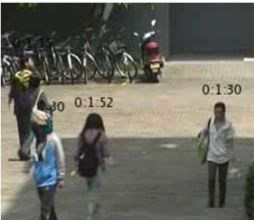
\includegraphics[width=0.2\linewidth]{ext-li02.png}
	}
	\subfloat[]
	{
		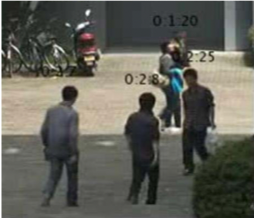
\includegraphics[width=0.2\linewidth]{ext-li03.png}
	}
	\subfloat[]
	{
		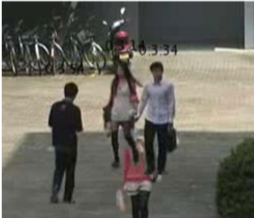
\includegraphics[width=0.2\linewidth]{ext-li04.png}
	}
	\\
	\subfloat[]
	{
		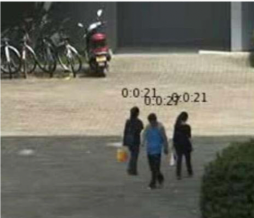
\includegraphics[width=0.2\linewidth]{ext-li05.png}
	}
	\subfloat[]
	{
		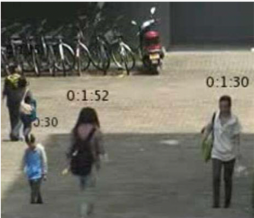
\includegraphics[width=0.2\linewidth]{ext-li06.png}
	}
	\subfloat[]
	{
		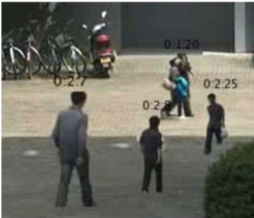
\includegraphics[width=0.2\linewidth]{ext-li07.png}
	}
	\subfloat[]
	{
		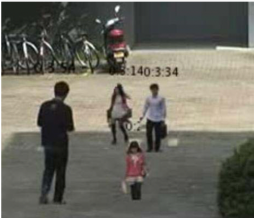
\includegraphics[width=0.2\linewidth]{ext-li08.png}
	}
	\caption{Synopsis results by scaling down objects~\cite{Li2016}. Because object sizes are not consistent and matched with the context, the results are visually uncomfortable.}
	\label{fig:Li}
\end{figure}

One of the big hurdles for video synopsis is that it works poorly on very crowded scenes. There are two approaches to solve the problem by 1) scaling down object sizes~\cite{Li2016} and 2) rearranging objects in both spatial and temporal domain~\cite{Nie2014}. As illustrated in \Cref{fig:Li}, reducing size of the objects can produce the less complicated condensed video and can have more objects in the scene simultaneously. However, as we can see in the results, scaled objects are visually awkward and some interactions between the objects are hard to understand. On the other hand, Li~\etal~\cite{Li2016} solve the problem by generating expanded background images and rearranging object tubes in spatio-temporal domain. As shown in \Cref{fig:Nie}, the background images have synthetically generated regions; the width of the sidewalk in the original image has been expanded to triple. Then, the algorithm utilizes such regions to reduce a complexity of the scene. It can produces descent results when the many objects in the scene walk along the same path. However, since generating the synthetic background image is not a straightforward task, the algorithm cannot be applied to videos having complex real-world scenes. In addition, as similar to the work of Nie~\etal~\cite{Nie2014}, the user has a chance to miss importance interactions between the objects.

\begin{figure}
	\centering
	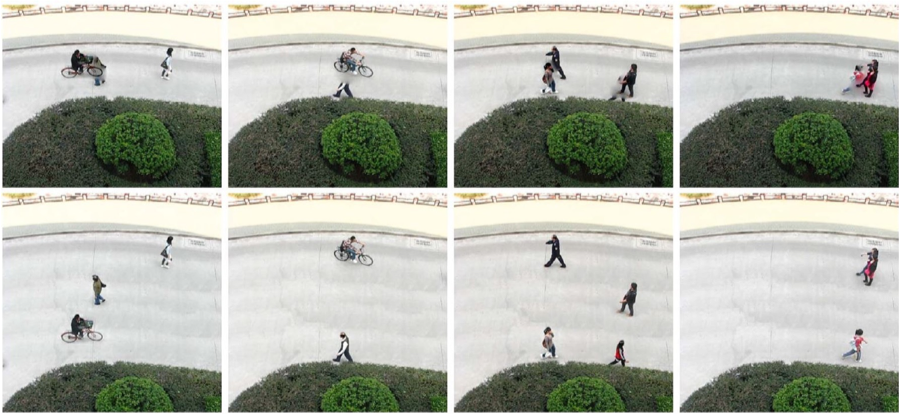
\includegraphics[width=\linewidth]{ext-nie.png}
	\caption{Result of object rearrangements in both spatial and temporal domains~\cite{Nie2014}. Images in the first row are from the input videos and synopsis results are presented in the second row. As we can see in the figure, width of the sidewalk has been expanded to triple, so that more objects can be displayed at the single frame simultaneously.}
	\label{fig:Nie}
\end{figure}

For the online video synopsis, six studies have been published in recent years. At first, the tube rearrangement algorithm inspired by the video game Tetris~\cite{Feng2012} has been developed. In the subsequent study~\cite{Zhu2015}, the high-performance online video synopsis framework which utilizes GPU and parallel processing to improve throughput of the system has been introduced. To apply the concept of Tetris to solve the video synopsis problem, two level cache condensed spaces (L1 and L2) are utilized. The L1 cache is the space, where starting labels of the objects are optimized. If the L1 cache space is filled enough with rearranged object tubes, the algorithm generates a portion of the synopsis video. On the other hand, L2 space is to hold tails of the object tubes which cannot be placed at L1 space completely. Since the portion of the condensed video is generated only when the L1 space is packed with objects, the length of the resulting video is changed according to the contents of the original video.

\begin{figure}
	\centering
	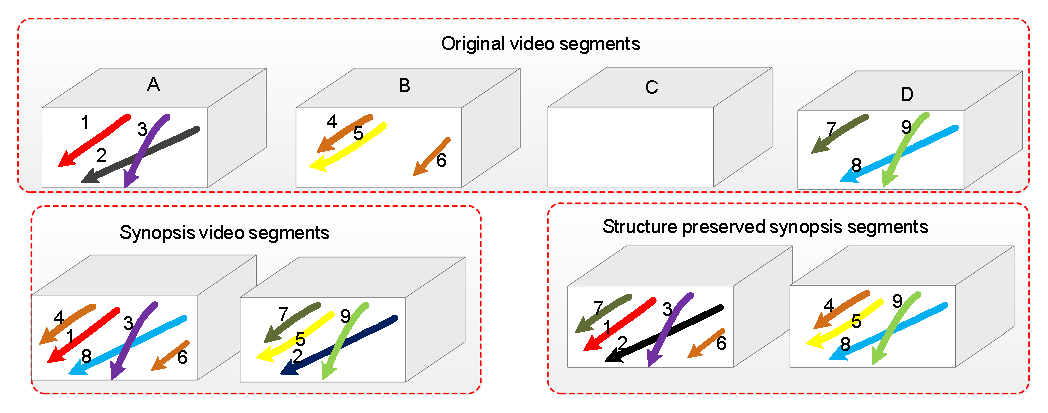
\includegraphics[width=\linewidth]{ext-fu.eps}
	\caption{Concept of the structure preserved video synopsis~\cite{Fu2014}. Objects have strong interactions in the original videos are also grouped together in the synopsis video.}
	\label{fig:Fu}
\end{figure}

Fu~\etal~\cite{Fu2014} try to keep interactions between the objects from being broken in the condensed video generated by the online framework. To achieve the objective, they consider motion proximity and interaction of objects. Simply said, the objects which are close each other and have similar motions are more likely to have low pairwise energies. The conceptual diagram of the structure preserved synopsis is illustrated in \Cref{fig:Fu}. Apart from the importance of preserving the motion structure between the objects, it adds computational burden for calculating pairwise energy terms. Even though the online video synopsis frameworks has fewer energy terms to consider than the offline framework, such drawback is not desirable to improve the throughput or latency of the system.

%A summary of the recent advances in video synopsis is presented as follows. Nie~\etal~\cite{Nie2014} rearrange object tubes in both temporal and spatial domain to generate more condensed videos. Zhu~\etal~\cite{Zhu2014} and Mahapatra~\etal~\cite{Mahapatra2016} extend the concept of video synopsis to the multi-camera network. Wang~\etal~\cite{Wang2013} and Zhong~\etal~\cite{Zhong2014} utilize the compressed domain to generate synopsis videos efficiently. X. Li~\etal~\cite{Li2016a} scale down object sizes to reduce collisions in the synopsis video. Z. Li~\etal~\cite{Li2009} and K. Li~\etal~\cite{Li2016} introduce a seam carving method to remove redundant information from the original video.

\section{Dissertation overview}
\label{sec:intro:overview}
The rest of the dissertation is organized as follows. \Cref{sec:basic_form} introduces the problem formulation of video synopsis and details of the proposed tube rearrangement algorithm are described in \Cref{sec:proposed}. \Cref{sec:framework} contains explanations of other components that the online video synopsis consists of. \Cref{sec:exp} presents experimental results, and the dissertation is concluded in \Cref{sec:conc}.

\chapter{Problem formulation of video synopsis}
\label{sec:basic_form}

In this chapter, the problem formulation of video synopsis introduced in the pioneering works~\cite{Rav-Acha2006,Pritch2007,Pritch2008} is described to show which part of the formulation has to be changed to apply parallel processing. In addition, the reason why online video synopsis mainly considers collision energy is explained in detail.

As in \Cref{fig:Rav-Acha,fig:video_synopsis_2d}, a principal objective of video synopsis is shortening length of the input video by relocating object tubes in temporal domain. In other words, we try to find the best combination of object tubes' starting positions in temporal domain (starting labels). In the field of video surveillance, a definition of the best combination can be different from specific applications. However, based on the paper of Pritch~\etal~\cite{Pritch2008}, the condensed video with the best starting label combination should have following characteristics.
\begin{itemize}
\item Objects of interests should be appeared in the condensed video.
\item Rearranged object tubes should seamlessly rendered in the condensed video.
\item The condensed video has significantly shorter length than the input video.
\item Dynamics of objects or interactions between the objects should be understood in the condensed video.
\end{itemize}
To achieve the characteristics, the batch video synopsis~\cite{Pritch2008} utilizes four energy terms as described in \Cref{sec:intro}: activity, background consistency, collision, and temporal consistency. The order of the energy terms are matched with that of the characteristics.

\begin{figure}
	\begin{center}
		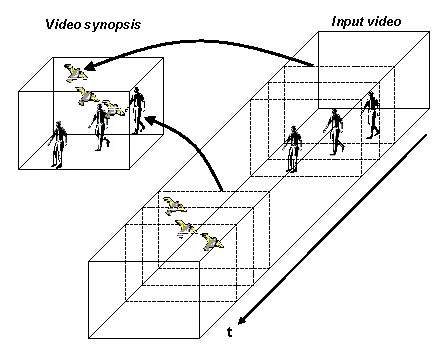
\includegraphics[width=\linewidth]{ext-rav-acha.eps}
	\end{center}
	\caption{Concept diagram of video synopsis~\cite{Rav-Acha2006}. The bird and man appeared at different time in the original video are rearranged in temporal domain, and then displayed simultaneously in the condensed video.}
	\label{fig:Rav-Acha}
\end{figure}

\begin{figure}
	\begin{center}
		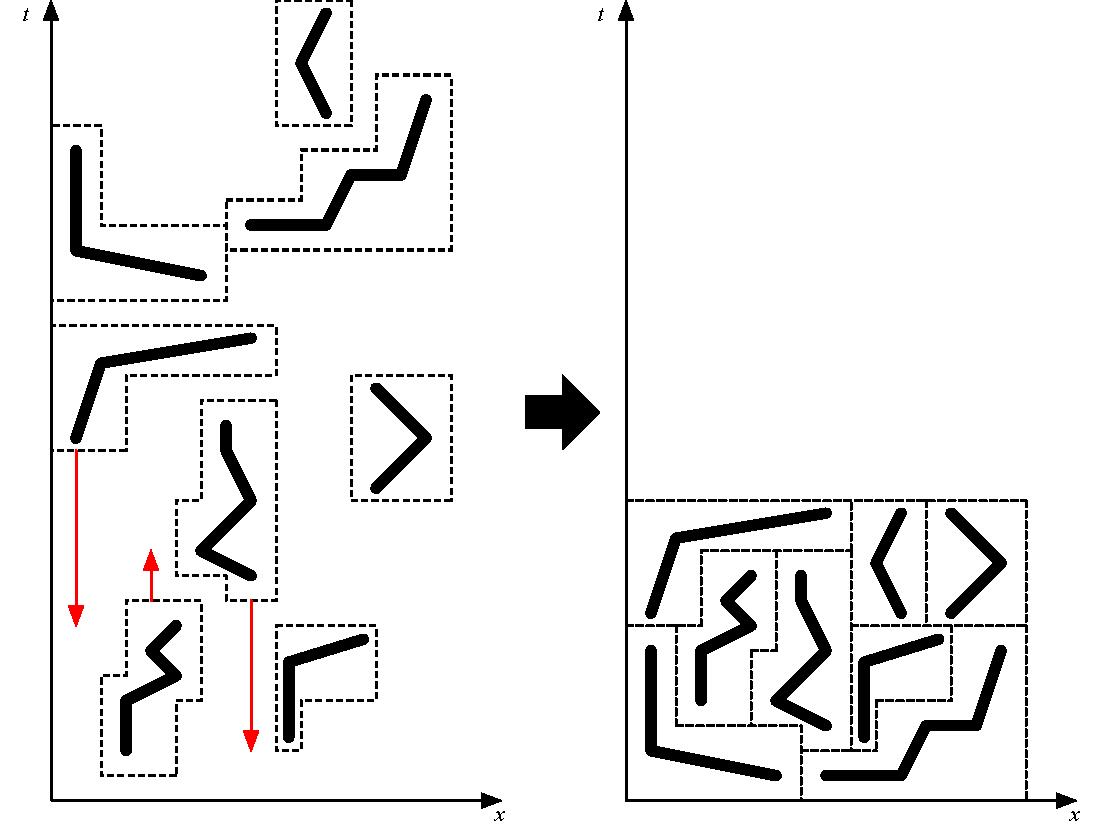
\includegraphics[width=\linewidth]{video_synopsis_2d.pdf}
	\end{center}
	\caption{Example of the object tube rearrangement in 2D space. Red arrows indicate some offsets of the starting labels for better understanding of the tube rearrangement process. We can see that after the tube rearrangement, the length of the condensed video becomes much shorter than that of the original.}
	\label{fig:video_synopsis_2d}
\end{figure}

Assume that $L=\{l_0,...,l_N\}$ is a set of starting labels for $N$ object tubes; then, an objective function $E(L)$ can be defined as
\begin{equation}
\label{eq:basic_form}
E(L)=\sum_{l_i \in L} \left( E_a(l_i) + \gamma E_s(l_i) \right) + \sum_{l_i,l_j \in L} \left( \alpha E_t(l_i, l_j) + \beta E_c(l_i, l_j) \right),
\end{equation}
where $E_a$, $E_s$, $E_t$, and $E_c$ are activity, background consistency, temporal consistency, and collision energies, respectively. In addition, $\alpha$, $\beta$, and $\gamma$ are weighting parameters for controlling importance between the energies.

\section{Activity energy}
At first, $E_a$ defines which object tubes should be appeared in the condensed video. One example of $E_a$ is
\begin{equation}
\label{eq:activity}
E_a(l_i) =
\begin{cases}
\sum_{x,y,t} \chi_i (x,y,t) & l_i \in L_e \\
0 & \rm{otherwise},
\end{cases}
\end{equation}
where $l_i$ and $\chi_i (x,y,t)$ are the starting label and the characteristic function of the $i^{\rm{th}}$ object tube, respectively. Due to the condition ($l_i \in L_e$) in (\ref{eq:activity}), the only characteristic function of the object tube whose starting label belongs to $L_e$ is added to $E_a$. The set $L_e$ contains starting labels of the objects not included in the condensed video. Therefore, the role of $E_a$ is penalizing exclusions of the object tubes. On the other hand, $\chi (x,y,t)$ represents the importance of the object tube. If the characteristic function of one object has larger values than that of the others, the object is more likely to be included in the resulting video. In the original work of video synopsis~\cite{Rav-Acha2006,Pritch2007,Pritch2008}, $\chi_i (x,y,t)$ is defined as
\begin{equation}
\label{eq:char_func}
\chi_i(x,y,t)=
\begin{cases}
\norm{I_i(x,y,t)-B(x,y,t)} & t \in t_i\\
0 & \rm{otherwise},
\end{cases}
\end{equation}
where $I_i(x,y,t)$ is a foreground pixel of $i^{\rm{th}}$ object and $B(x,y,t)$ is a respective background pixel, and $t_i$ is a period of time in frames indicating the appearance of the object. Based on (\ref{eq:char_func}), the condensed video prefers the object tubes having distinctive colors as compared with the background. 

Defining a proper $E_a$ is important for processing the query of the video synopsis users, since it determines which objects will be included in the resulting video. However, we do not have to directly optimize $E_a$ because object filtering step prior to the optimization with specific conditions (e.g., colors, trajectories, object types, and etc) can do the same functionality.

\section{Time-lapse background generation}
Before moving on to the next energy term, how to generate time-lapse background is briefly explained. Since the main objective of video synopsis is condensing the contents of the original video, background information as well as foreground has be condensed too. If the input video is 12 hours long and the condensed video is 10 minutes long, time-lapse background can be generated by uniformly subsampling every 720th of original background images or we can use the adaptive sampling rate proportional to (or inverse proportional to) the number of objects in the current frame~\cite{Pritch2008}. An example of the time-lapse background generation is illustrated in \ref{}.

\section{Background consistency energy}
The role of the second energy term in (\ref{eq:basic_form}), $E_s$, is to seamlessly render the object tubes with the time-lapse background images. In the video synopsis framework, foreground pixels of the object tubes are stitched with the background images to generate the condensed video. During the stitching process, image blending algorithms (e.g., Poisson image editing~\cite{Perez2003}) can be used to smoothly blend the foreground and background pixels. However, inaccurate segmentation results of the foreground or foreground and background pixels from different time of day can cause visually unappealing results as shown in \ref{}. $E_s$ is defined to penalize such situation.
\begin{equation}
\label{eq:bg_consistency}
E_s(l_i)=\sum_{x,y \in \sigma_i,t}\norm{I_i(x,y,t)-B_t(x,y,t)},
\end{equation}
where $\sigma_i$ is a set of boundary pixels for the $i^{\rm{th}}$ object and $B_t(x,y,t)$ is a pixel of the time-lapse background. To obtain $\sigma_i$, we can apply morphological dilation to the foreground mask of the $i^{\rm{th}}$ object and subtract it from the original. Based on (\ref{eq:bg_consistency}), the object appeared in the midnight are more likely to be appeared at night-part of the time-lapse background.

In the online video synopsis framework, object tube extraction, time-lapse background generation, and foreground-background stitching are conducted in real-time; therefore, foreground and background pixels are from the similar time of day. Therefore, online video synopsis has less reason to consider $E_s$ during the optimization.

\section{Temporal consistency energy}
The temporal consistency energy, $E_t$, is designed to keep chronological orders between the object tubes in the original video. If the condensed video contains chronological disorders between the tubes, we may miss the important interaction between the objects presented in the original video. Prior to further discussion about $E_t$, we need to define a probability of the interaction between the two object tubes first. If the objects share common time periods in the original video $(t_i \cap t_j \neq \emptyset)$, the probability becomes
\begin{equation}
\label{eq:prob_share_time}
p_I(i, j) = 
\exp\left(-\min_{t \in t_i \cap t_j} \frac{d(i,j,t)}{\sigma_s}\right),
\end{equation}
where $d(i,j,t)$ is a Euclidean distance between the closest pixels of $i^{\rm{th}}$ and $j^{\rm{th}}$ objects in frame $t$ and $\sigma_s$ is a parameter for adjusting a spatial range of the interaction. Based on (\ref{eq:prob_share_time}), a pair of the objects spatially adjacent to each other is more likely to have interactions between them.

On the other hand, if the objects do not have any overlap in the temporal domain of the original video, $p_I(i,j)$ is defined as
\begin{equation}
\label{eq:prob_not_share_time}
p_I(i,j)=\exp\left(-\frac{l_j - (l_i + T_i)}{\sigma_t}\right),
\end{equation}
where $T_i$ is the number of frames in the $i^{\rm{th}}$ object tube and $\sigma_t$ determines a temporal proximity between the objects. In addition, (\ref{eq:prob_not_share_time}) is defined on the assumption that the $i^{\rm{th}}$ object appears earlier than the $j^{\rm{th}}$ object in the input video ($l_i + T_i < l_j$). Therefore, the object tubes located far from each other in temporal domain are less likely to have interactions.

In summary, (\ref{eq:prob_share_time}) and (\ref{eq:prob_not_share_time}) encode the idea that objects close in spatio-temporal domain have strong interactions. Based on the two equations, we can define $E_t$ to keep chronological orders between the objects when generating the condensed video.
\begin{equation}
\label{eq:Et}
E_t(i,j)=
p_I(i, j) \cdot
\begin{cases}
0 & \hat{l}_i - \hat{l}_j = l_i - l_j \\
C & \rm{otherwise},
\end{cases}
\end{equation}
where $\hat{l}$ indicates a starting label of the object in the input video and $C$ is a large constant value to penalize the objects having temporal inconsistencies. 

Since the behavior of the equation (\ref{eq:Et}) is not straightforward, detail explanations will be given through examples. Assume that two objects are close in spatio-temporal domain of the original video. In this case, $E_t$ of two objects becomes very large (due to $C$), when their relative starting label in the condensed video ($l_i - l_j$) is not exactly same as in the input video ($\hat{l}_i - \hat{l}_j$). Conversely, the objects far from each other in spatio-temporal domain have a low penalty for violating the condition ($\hat{l}_i - \hat{l}_j = l_i - l_j$), because their $p_I$ has a small value.

As similar to $E_s$, the role of $E_t$ is not significant in online video synopsis. Recent online video synopsis frameworks~\cite{Fu2014,He2017} maintain a queue of object tubes and the queue grows as new object tube is extracted in the input video. When the size of the queue exceeds a certain threshold $K$, framework generates a partial condensed video with $K$ object tubes, and then removes the first $K$ objects from the queue. Based on the framework, chronological disorders only can be presented when the objects are in the same part of the condensed video. Even if the objects are optimized together to generate a same part of the resulting synopsis video, their temporal inconsistencies are negligible, because their relative spatio-temporal distance is small. In consequence, the one and only energy term to optimize in online video synopsis is the collision energy.

\section{Collision energy}
The key role of $E_c$ is to prevent the resulting synopsis video from becoming crowded. During the video synopsis process, the objects from different time periods in the input video are displayed simultaneously in the same scene of the condensed video. In this case, pixel overlaps between the objects make us difficult to understand the context of the synopsis video. To penalize such situation through $E_c$, a degree of collision between the objects is defined as
\begin{equation}
\label{eq:Ec}
E_c(l_i,l_j)=\sum_{x,y,t \in t_i \cap t_j} \chi_i(x,y,t) \chi_j(x,y,t).
\end{equation}

Based on (\ref{eq:Ec}), a collision between two objects having distinctive colors from the background is considered more seriously. However, this definition of $E_c$ is computationally expensive due to $\chi(x,y,t)$. Therefore, in this dissertation, the multiplication of two characteristic functions is replaced with the intersection over union (IoU) between two bounding boxes of the objects.
\begin{equation}
\label{eq:EcApprox}
E_c(l_i,l_j)=\sum_{x,y,t \in t_i \cap t_j} IoU \left( B_i(t),B_j(t) \right),
\end{equation}
\begin{equation}
IoU(B_i,B_j)=\frac{B_i \cap B_j}{B_i \cup B_j},
\end{equation}
where $B_i(t)$ and $B_j(t)$ are bounding boxes of $i^{\rm{th}}$ and $j^{\rm{th}}$ objects at frame $t$, respectively. Since the bounding box does not represent an exact location of the object, (\ref{eq:EcApprox}) can be thought as an approximated version of (\ref{eq:Ec}).

\section{Computational bottleneck}
In (\ref{eq:basic_form}), we should note that energies can be categorized into two groups regarding the number of required parameters: unary and pairwise. Activity and background consistency only requires a single object tube to calculate the energies; on the other hand, remaining energies require two object tubes for the calculation. When the number of objects to optimize increases, pairwise energy terms become a bottleneck of the computation. Since $E_s$ is not the main concern of online video synopsis, $E_c$ becomes the one and only issue for the computational burden. As described in \Cref{sec:intro:related}, recent studies of video synopsis~\cite{He2017} utilize different calculations of $E_c$, but their definitions of the collision energy are not suitable for parallel processing. In the following section, a new representation of the object tube named as an occupation matrix which has a suitable form for concurrent computation of $E_c$ will be introduced.

\begin{sidewaysfigure}
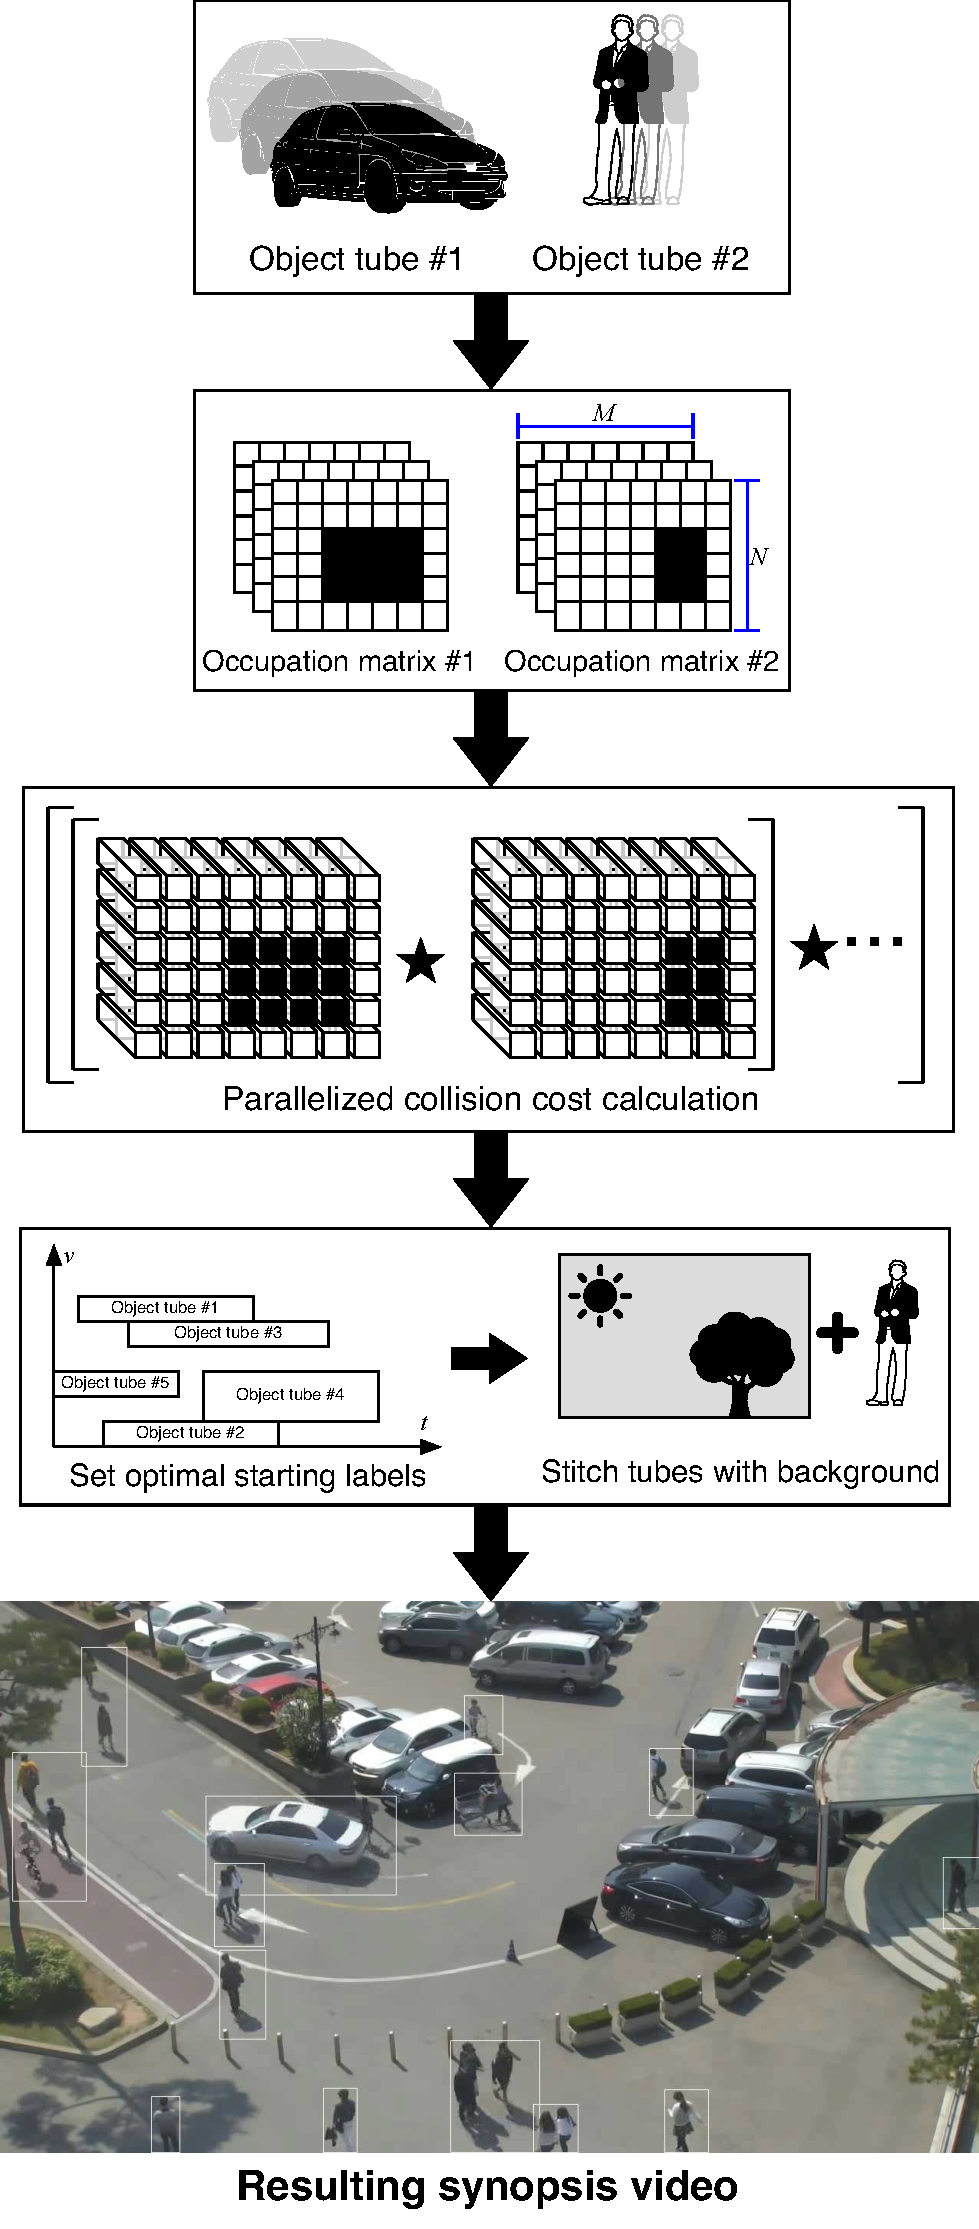
\includegraphics[width=\linewidth]{flowchart.pdf}
\caption{Flowchart of the proposed online video synopsis framework. At the beginning, foreground of the object tube is reshaped into the 3D occupation matrix. We use this matrix representation to calculate the collision energy fast in conjunction with parallel processing and Fourier transform. Afterwards, we determine optimal starting labels for tubes and stitch tubes with the background to generate a resulting synopsis video. Illustrations of man and vehicle in this figure are created by Lluisa Iborra and Yasser Megahed from the Noun Project.}
\label{fig:flowchart}
\end{sidewaysfigure}

\chapter{Proposed tube rearrangement}
\label{sec:proposed}
In this chapter, $E_c$ is reformulated using the occupation matrix and an efficient tube rearrangement algorithm for optimizing the objective function is proposed. In addition, two types of the occupation matrix (binary and probabilistic) are introduced and their characteristics are explained in detail. A flowchart of the proposed online video synopsis framework including the tube rearrangement algorithm is illustrated in \Cref{fig:flowchart}.

\section{Occupation matrix generation}
\label{sec:proposed:occ}
Each element of the occupation matrix $\textbf{M}_i (u,v,t)$ is either from Boolean or continuous domain, and represents the probability of existence for $i^{\rm{th}}$ object tube at position $(u,v)$ and time $t$ of a video whose spatial resolution is $\mathcal{H} \times \mathcal{W}$. The $i^{\rm{th}}$ occupation matrix $\textbf{M}_i$ is then formed by stacking resized binary foreground masks of the object over multiple frames. The resized foreground mask has $\mathcal{M} \times \mathcal{N}$ resolution, where $\mathcal{M}$ and $\mathcal{N}$ have much smaller values than the width and height of the original video ($\mathcal{M} \ll \mathcal{H}$ and $\mathcal{N} \ll \mathcal{W}$). In this dissertation, two strategies of resizing will be introduced in following subsections and they determine the type of resulting occupation matrix: binary and probabilistic.

\subsection{Binary occupation matrix}
\label{sec:proposed:occ:binary}
The binary occupation matrix $\textbf{M}^b$ does not allow gray area value to represent the existence of objects; it can only have 1s and 0s. Assume that the foreground mask of the $i^{\rm{th}}$ object is denoted as $\textbf{F}_i(x,y,t) \in \mathbb{B}$; then, $\textbf{M}_i^b(u,v,t)$ is defined as
\begin{equation}
\label{eq:bin_occ}
\textbf{M}_i^b(u,v,t)=
\begin{cases}
1 & \sum_{(x,y) \in C(u,v)}\textbf{F}_i(x,y,t) \neq 0 \\
0 & \rm{otherwise},
\end{cases}
\end{equation}
where $C(u,v)$ is a set of 2D coordinates $(x,y)$. Based on (\ref{eq:bin_occ}), to calculate a single element of $\textbf{M}_i^b$, we need to examine the values of $\textbf{F}_i$ for every coordinate in $C(u,v)$. The definition of $C(u,v)$ is given by
\begin{equation}
C(u,v)=\left\{ (x,y) \mid x \in X(u), y \in Y(v) \right\},
\end{equation}
where $X(u)$ and $Y(v)$ are sets of $x$ and $y$ coordinates, respectively.
\begin{equation}
X(u)=\left\{ x \;\middle|\; \round*{\frac{\mathcal{W}}{\mathcal{N}}u} \leq x < \round*{\frac{\mathcal{W}}{\mathcal{N}}\left( u + 1 \right)} \right\},
\end{equation}
\begin{equation}
Y(v)=\left\{ y \;\middle|\; \round*{\frac{\mathcal{H}}{\mathcal{M}}v} \leq y < \round*{\frac{\mathcal{H}}{\mathcal{M}}\left( v + 1 \right)} \right\}.
\end{equation}

Due to the condition $\left( \sum_{(x,y) \in C(u,v)}\textbf{F}_i(x,y,t) \neq 0 \right)$ in (\ref{eq:bin_occ}), even a single pixel of $\textbf{F}_i(x,y,t)$ can produce a response in $\textbf{M}_i^b(u,v,t)$. Therefore, $\textbf{M}_i^b$ exaggerates the occupation region of the object tube in the video sequence. An example of the binary occupation matrix generation is depicted in \Cref{fig:bin_occ}.

\begin{figure}
	\begin{center}
		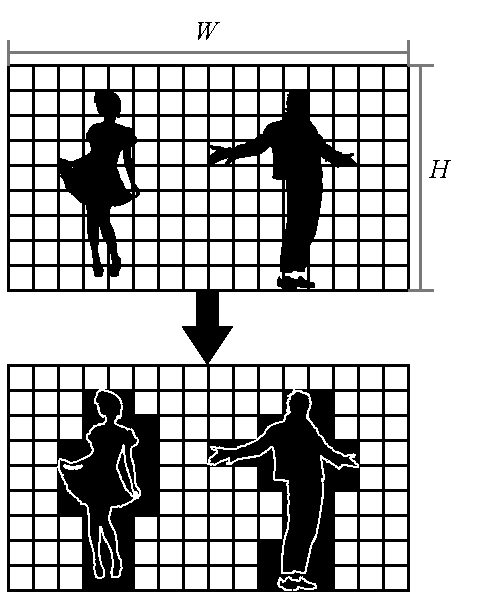
\includegraphics[width=0.7\linewidth]{bin-occ.pdf}
	\end{center}
	\caption{Example of the binary occupation matrix generation when $\mathcal{M}\times\mathcal{N}=9\times16$. The foreground and background of the object are represented in black and white, respectively. Dotted lines in the figure are depicted to show contours of the original object for the readers. Illustrations of the woman and man in this figure are created by Nataliia Lytvyn and Ludovic Gicqueau from the Noun Project, respectively.}
	\label{fig:bin_occ}
\end{figure}

\subsection{Probabilistic occupation matrix}
\label{sec:proposed:occ:prob}
Since the probabilistic occupation matrix $\textbf{M}_i^p$ represents the existence of the object tube with continuous values, it can provide more precise information than $\textbf{M}_i^b$. Each element of $\textbf{M}_i^p$ is calculated as
\begin{equation}
\label{eq:prob_occ}
\textbf{M}_i^p(u,v,t)= \frac{\sum_{(x,y) \in C(u,v)}\textbf{F}_i(x,y,t)}{|C(u,v)|}.
\end{equation}
where $|C(u,v)|$ is a cardinality of $C(u,v)$. In most cases, where $\mathcal{W}/\mathcal{N} \in \mathbb{N}$ and $\mathcal{H}/\mathcal{M} \in \mathbb{N}$, $|C(u,v)|$ becomes a constant value.

%\subsection{Binary vs. probabilistic}
%The main role of the occupation matrix is to provide a spatial approximation of $\textbf{F}_i$. Since both representations can achieve the objective, selecting the type of the occupation matrix is same as considering the trade-off between the accuracy and computation time. In general, using $\textbf{M}_i^p$ can produce more compact synopsis video with more computational burden. On the other hand, the scene in the condensed video based on $\textbf{M}_i^b$ is less complex and can be generated with less computation. Quantitative evaluations regarding the type of the occupation matrix will be given in \Cref{sec:exp}.

\section{Objective function}
For the next step, the collision energy is reformulated with the occupation matrix and a new energy term $E_l$ is introduced to penalize a long condensed video. Then, the final objective function of the proposed tube rearrangement algorithm is defined by considering both $E_c$ and $E_l$. 
\begin{sidewaysfigure}
	\centering
	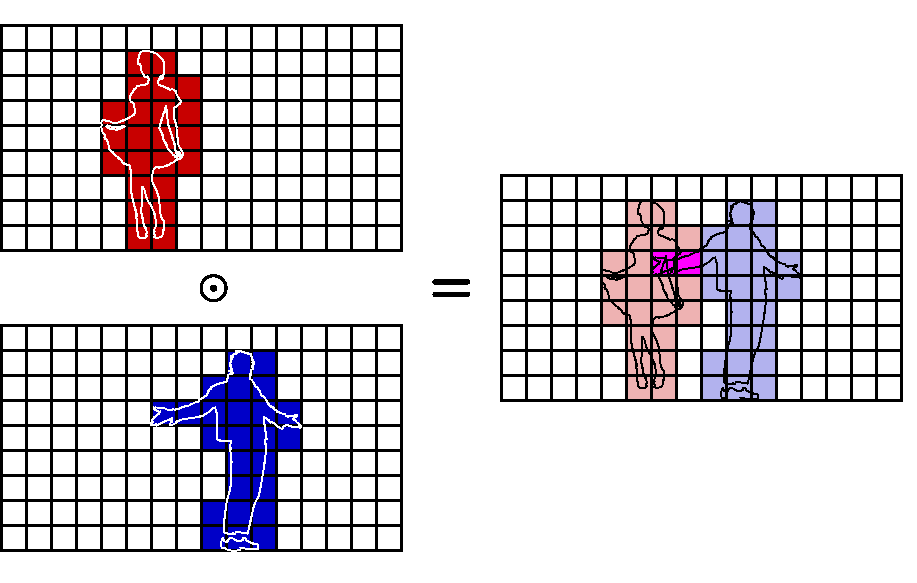
\includegraphics[width=0.8\linewidth]{hadamard-prod.pdf}
	\caption{Example calculation of reformulated collision energy $E_c$ with two binary occupation matrices. Occupied elements in the matrix are colored in red and blue. After the element-wise multiplication, we can see that the objects have two collided elements colored in magenta. In this figure, $\odot$ is an operator for the element-wise multiplication, also known as Hadamard product.}
	\label{fig:hadamard_prod}
\end{sidewaysfigure}
\subsection{Reformulated collision energy}
The motivation behind the reformulation of $E_c$ is that the degree of collision between the objects at a certain frame can be calculated as a sum of the element-wise multiplication of two occupation matrices. An example of this computation is depicted in \Cref{fig:hadamard_prod} and the redefined $E_c(l_i,l_j)$ is given by
\begin{equation}
\label{eq:EcNew}
E_c(l_i,l_j) = \sum_{u=1}^{\mathcal{M}}\sum_{v=1}^{\mathcal{N}}\sum_{t=t_{\rm{min}}}^{t_{\rm{max}}} \textbf{M}_i(u,v,t)\textbf{M}_j(u,v,t),
\end{equation}
where $t_{\rm{min}}$ and $t_{\rm{max}}$ are minimum and maximum values of the overlapped temporal domain. Detailed calculations of $t_{\rm{min}}$ and $t_{\rm{max}}$ are
\begin{equation}
\label{eq:t_min}
t_{\rm{min}} = \max(l_i, l_j),
\end{equation}
\begin{equation}
\label{eq:t_max}
t_{\rm{max}} = \min(T_i + l_i, T_j + l_j),
\end{equation}
where $T_i$ and $T_j$ are frame lengths of the $i^{\rm{th}}$ and $j^{\rm{th}}$ object tubes, respectively.

\subsection{Length energy}
Apart from the existing video synopsis frameworks using the fixed length of the synopsis video~\cite{}, the proposed framework adaptively adjusts the length of the condensed video by considering both compactness and complexity. In this regard, the length energy $E_l (l_i,l_j)$ is defined as the frame length of the synopsis video when two object tubes have starting labels of $l_i$ and $l_j$.
\begin{equation}
\label{eq:El}
E_l(l_i, l_j) = \max(T_i + l_i, T_j + l_j) - \min(l_i, l_j).
\end{equation}
An objective function $E(l_i,l_j)$ is calculated as a weighted sum of the collision and length energies.
\begin{equation}
\label{eq:obj_func}
E(l_i, l_j) = E_c(l_i, l_j) + \lambda E_l(l_i, l_j),
\end{equation}
where $\lambda$ is a weighting parameter adjusting the importance of the length energy. In general, the larger $\lambda$ generates the shorter but more complex synopsis video; on the other hand, the smaller $\lambda$ produces the longer but less confused condensed video.

\section{Optimizing objective function}
As in other online video synopsis algorithms~\cite{Fu2014,Zhu2015,He2017}, the proposed tube rearrangement algorithm adopts the stepwise optimization strategy; therefore, starting labels of the object tubes are determined one by one through iterations. At the $i^{\rm{th}}$ iteration of the optimization, the starting label of $i^{\rm{th}}$ object tube $l_i$ is determined as
\begin{equation}
\label{eq:starting_label}
l_i = \arg\min_l E(l, L_{i-1}) \textrm{ subject to } l_i \geq 0,
\end{equation}
where $L_{i-1} = \{ {l}_{1},...,{l}_{i-1} \}$ is a set of starting labels determined after $i-1$ iterations. A constraint to the optimization ${l}_{i} \geq 0$ is used to alleviate chronological disorder in the synopsis video. In other words, since a negative $l_i$ means that $i^{\rm{th}}$ tube appear prior to the first tube in the synopsis video, preventing such case increases a chance to keep chronological order of the tubes. 

Due to the stepwise optimization strategy, one of two input arguments for $E$ in (\ref{eq:starting_label}) becomes $L_{i-1}$ instead of a single label as described in (\ref{eq:obj_func}). In consequence, slight modifications of (\ref{eq:EcNew}) and (\ref{eq:El}) are necessary. For the stepwise optimization, the calculation of $E_c$ is modified as
\begin{equation}
\label{eq:EcStepwise}
E_c(l_i,L_{i-1}) = \sum_{u=1}^{\mathcal{M}}\sum_{v=1}^{\mathcal{N}}\sum_{t=t_{\rm{min}}^{*}}^{t_{\rm{max}}^{*}} \textbf{M}_i(u,v,t)\textbf{M}_{i-1}^{*}(u,v,t),
\end{equation}
where $\textbf{M}_{i-1}^{*}$ is an accumulated occupation matrix for $i-1$ iterations, and $t_{\rm{min}}^{*}$ and $t_{\rm{max}}^{*}$ are minimum and maximum bounds of shared temporal domain between $\textbf{M}_i$ and $\textbf{M}_{i-1}^{*}$. Moreover, each element of $\textbf{M}_{i-1}^{*}$ is defined in the recurrence relation as
\begin{equation}
\label{eq:acc_occ}
\textbf{M}_{i-1}^{*}(u, v, t) = \textbf{M}_{i-1}(u, v, t - l_{i-1}) + \textbf{M}_{i-2}^{*}(u, v, l_{i-2}^{*}),
\end{equation}
where $l_{i-2}^{*} = \min L_{i-2}$. For the initial condition of~(\ref{eq:acc_occ}), $\textbf{M}_{1}^{*} = \textbf{M}_{1}$ and $l_{1}^{*} = l_{1} = 0$ are used. Formal definitions of $t_{\rm{min}}^{*}$ and $t_{\rm{max}}^{*}$ are
\begin{equation}
t_{\rm{min}}^{*} = \max(l_i, l_{i-1}^{*})
\end{equation}
and
\begin{equation}
t_{\rm{max}}^{*} = \min(T_i + l_i, T_{i-1}^{*} + l_{i-1}^{*}),
\end{equation}
where $T_{i-1}^{*}$ is a frame length of $\textbf{M}_{i-1}^{*}$. The length energy for the stepwise optimization is defined as
\begin{equation}
E_l(l_i,L_{i-1})=\max(T_i+l_i,T_{i-1}^{*}+l_{i-1}^{*})-\min(l_i,l_{i-1}^{*}).
\end{equation}
\subsection{Properties of accumulated occupation matrix}
For better understanding of the stepwise optimization process, we will discuss about properties of the accumulated occupation matrix $\textbf{M}^{*}$. According to the type, the occupation matrix $\textbf{M}$ can have either Boolean or continuous values in the range from 0 to 1. On the other hand, $\textbf{M}^{*}$ is computed by adding two matrices as described in (\ref{eq:acc_occ}); therefore, each element of $\textbf{M}^{*}$ belongs to either $\mathbb{N}_{0}$ or $\mathbb{R}_{\geq 0}=\left\{ x \in \mathbb{R} \mid x \geq 0  \right\}$. By utilizing $\textbf{M}^{*}$, we can represent occupation and collision states of more than two objects on the single matrix.

\section{Parallelized optimization}
Even though $\textbf{M}$ provides an efficient way of representing the object tubes and $E_c$ can be computed easily with the element-wise multiplication, optimization of $E_c$ can further be accelerated by using both parallel processing and cross-correlation of two occupation matrices in the temporal domain. Prior to define the cross-correlation, assume that two occupation matrices overlap by at least one frame in the temporal domain. Without this restriction, $E$ needs to be evaluated for every possible $l$ value. Then, the parallelized version of $E_c$ in (\ref{eq:EcStepwise}) is defined as
\begin{equation}
\label{eq:EcPP}
\begin{aligned}
E_c(l_i, L_{i-1}) = \sum_{u=1}^{\mathcal{M}} \sum_{v=1}^{\mathcal{N}} \textbf{M}_{i} \star \textbf{M}_{i-1}^{*}(u, v, l_i - l_{i-1}^{*}) \\
= \sum_{u=1}^{\mathcal{M}} \sum_{v=1}^{\mathcal{N}} \sum_{t=-\infty}^{\infty} \textbf{M}_{i}\textbf{M}_{i-1}^{*}(u, v, t + l_i - l_{i-1}^{*}),
\end{aligned}
\end{equation}
where $\star$ is an operator for the cross-correlation.

The motivation behind the conversion from (\ref{eq:EcStepwise}) to (\ref{eq:EcPP}) is illustrated in \Cref{fig:Ec_motivation}. From (\ref{eq:EcStepwise}), if we take the spatial coordinate into the consideration first, the 3D element-wise multiplication can be thought as a series of 2D Hadamard products in temporal domain as shown in \Cref{fig:3d_hadamard}. On the other hand, if we consider the temporal domain first, the operation becomes $\mathcal{M} \times \mathcal{N}$ 1D cross-correlations as illustrated in \Cref{fig:1d_cross_corr}. This difference may seem to be minor but it is important when we consider some tricks to accelerate the operation. The computational burden of multiple 1D cross correlations can be reduced by fast Fourier Transform (FFT)~\cite{Oppenheim2009} in conjunction with parallel processing. A detailed procedure of the proposed tube rearrangement algorithm is presented in \Cref{alg:proposed}.
\begin{figure}
	\centering
	\subfloat[2D Hadamard products]
	{
		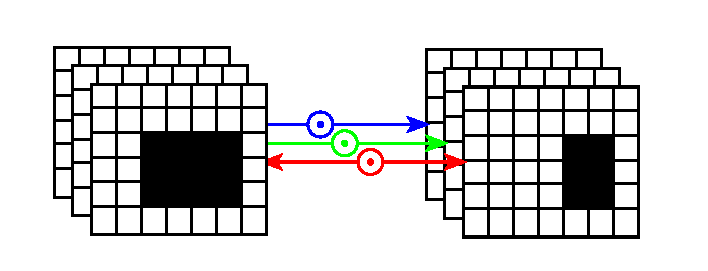
\includegraphics[width=0.9\linewidth]{3d-hadamard-prod.pdf}
		\label{fig:3d_hadamard}
	}
	\qquad
	\subfloat[1D cross-correlations]
	{
		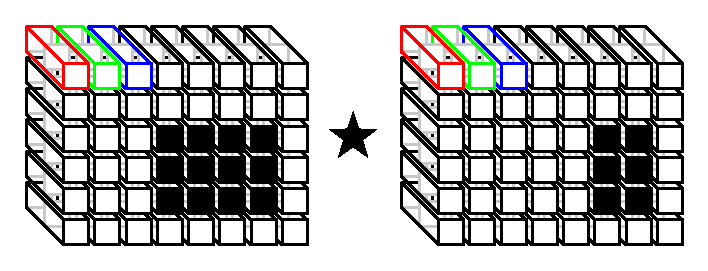
\includegraphics[width=0.9\linewidth]{1d-cross-corr.pdf}
		\label{fig:1d_cross_corr}
	}
	\caption{Two ways of calculating $E_c$. All of occupation matrices in this figure have $6 \times 8 \times 3$ spatio-temporal resolution. $E_c$ can be calculated by using \protect\subref{fig:3d_hadamard} Hadamard products between two sets of frames, and \protect\subref{fig:1d_cross_corr} 1D cross correlations between 48 pairs of 1D signals. Three primitive colors (red, green, and blue) in this figure is used to show example correspondences.}
	\label{fig:Ec_motivation}
\end{figure}
\begin{algorithm}[t]
	\caption{Proposed tube rearrangement algorithm}
	\label{alg:proposed}
	\begin{algorithmic}
		\REQUIRE $\textbf{M}_{i}, i = 1,...,N$
		\ENSURE $L_{N} = \{ l_{1},...,l_{N} \}$
		
		\STATE $\textbf{M}_{1}^{*} = \textbf{M}_{1}$, $l_{1}^{*} = l_{1} = 0$, $L_{1} = \{ l_{1} \}$
		
		\FOR {$i = 2$ to $N$}
		\STATE Calculate $\textbf{M}_{i} \star \textbf{M}_{i-1}^{*}$ using FFT and parallel processing
		\STATE Find a local optimum starting label $l_{i}$ by using~(\ref{eq:starting_label})
		\iffalse
		\STATE $l_{i} = \arg\min_{l} E(l, L_{i-1})$ subject to $l_{i} \geq 0$
		\fi
		\STATE Calculate $\textbf{M}_{i}^{*}$ from $\textbf{M}_{i}$ and $\textbf{M}_{i-1}^{*}$ by using~(\ref{eq:acc_occ})
		\iffalse
		\STATE $\textbf{M}_{i}^{*}(u, v, t) = \textbf{M}_{i}(u, v, t-l_{i}) + \textbf{M}_{i-1}^{*}(u, v, t-l_{i-1}^{*})$
		\fi
		\STATE $L_{i} = L_{i-1} \cup l_{i}$
		\STATE $l_{i}^{*} = \min L_{i}$
		\ENDFOR
		
		\RETURN $L_{N}$
	\end{algorithmic}
\end{algorithm}
\chapter{Online video synopsis framework}
\label{sec:framework}
The proposed tube rearrangement algorithm is based on the online framework. Similar to existing online frameworks~\cite{Fu2014,Zhu2015,He2017}, the proposed framework consists of four stages: background modeling, object tube generation, tube rearrangement, and object stitching. Among them, three components, except for the tube rearrangement, will be explained in detail.

\section{Background modeling}
Since this field of research has been studied for decades, there are numerous choices for modeling the background: Gaussian Mixture Models (GMM)~\cite{Zivkovic2004,Zivkovic2006}, ViBe variants~\cite{Barnich2009ViBe,Barnich2011ViBe,VanDroogenbroeck2012Background,VanDroogenbroeck2014ViBe}, SOBS~\cite{maddalena2008self,maddalena2012sobs}, non-parametric background modelings~\cite{Hofmann2012,Muchtar2018}, deep CNN based approaches~\cite{Patil2018,Lim2018}, and GAN based approaches~\cite{Bakkay2018,Sultana2019,Sakkos2019}. Among them, GMM introduced by Zivkovic~\cite{Zivkovic2004} is utilized in the framework, because OpenCV 3.0 or above supports the GPU accelerated implementation of the method.

\begin{comment}
According to the recent review literature~\cite{bouwmans2018deep}, apart from well-established statistical background modelings~\cite{Zivkovic2004,Zivkovic2006,Barnich2009ViBe,Barnich2011ViBe,VanDroogenbroeck2012Background,VanDroogenbroeck2014ViBe,Hofmann2012,Muchtar2018} and neural network based approaches~\cite{maddalena2008self,maddalena2012sobs}, deep learning based approaches become a main stream of the research. %and they can be categorized into two broad groups: convolutional neural networks (CNN)~\cite{Patil2018,Lim2018} and generative adversarial network (GAN)~\cite{Bakkay2018,Sultana2019,Sakkos2019}.
\begin{sidewaysfigure}
	\centering
	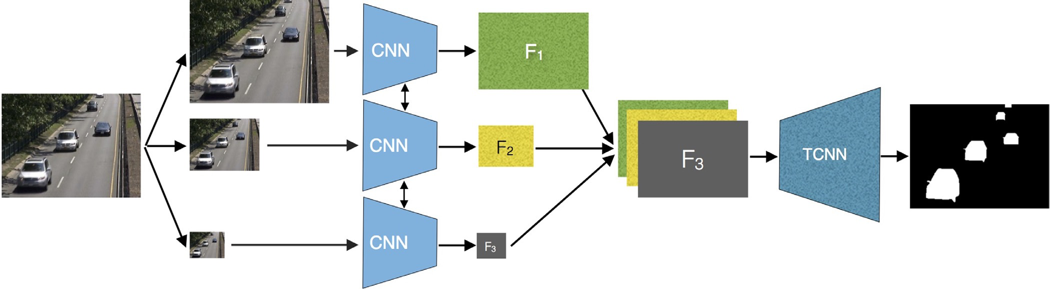
\includegraphics[width=0.8\linewidth]{bg_dcnn.png}
	\caption{Flowchart of foreground segmentation by Lim~\etal~\cite{Lim2018}. It follows the common process of the image segmentation, but its performance has been increased by incorporating feature maps from multiple scales.}
	\label{fig:bg_dcnn}
\end{sidewaysfigure}

\Cref{fig:bg_dcnn} shows a process of segmenting the foreground from the background introduced by Lim~\etal~\cite{Lim2018}. This process has a lot in common with image segmentation using CNN architecture~\cite{Long2015,chen2014semantic,chen2017rethinking,Zhao2017,chen2018deeplab,chen2018encoder}; encoder module is for extracting feature maps and decoder module is for compensating reduced spatial resolution. The key difference between the foreground and image segmentation is the number of output labels; the former produces only two labels while the latter discerns more than 20 labels for renowned PASCAL VOC 2012 dataset~\cite{Everingham15} and 30 labels for Cityscapes dataset targeted for the autonomous driving application~\cite{Cordts2016Cityscapes}.

\begin{figure}
	\centering
	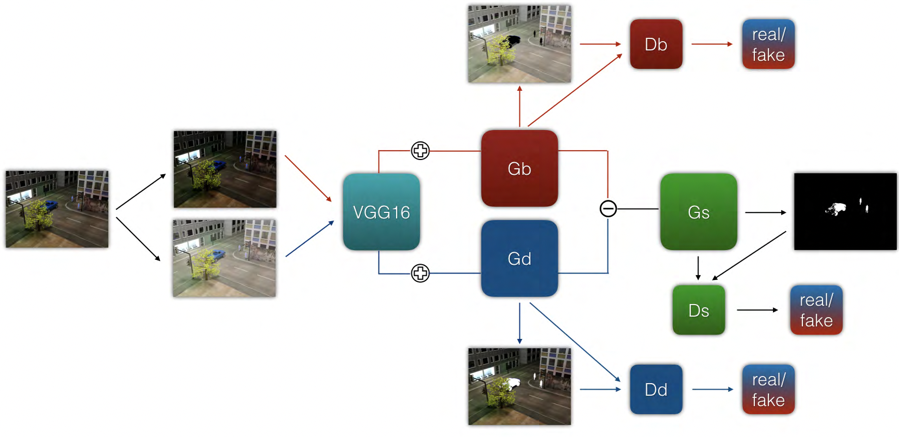
\includegraphics[width=\linewidth]{bg_gan.png}
	\caption{Recent framework of foreground segmentation via GAN~\cite{Sakkos2019}. It utilizes three generator-discriminator pairs to make foreground segmentation robust against extreme illumination changes. At first, input images undergo the gamma correction to make them in the extreme illumination condition. Red $G_b$ and $D_b$ boxes to generate synthetic bright images from dark images, and to discriminate the synthetic and original ones. On the other hand, blue $G_b$ and $D_b$ boxes do the same task for the bright images. Finally, by using the results of red and blue $G_b$, $G_s$ and $D_s$ are trained to generate and discriminate segmented foregrounds.}
	\label{fig:bg_gan}
\end{figure}
GAN is one of the most actively researched topics in the computer vision. Due to its intriguing idea, many researchers in different field of studies try to solve their problems by using GAN and the problem of modeling background is one of them~\cite{Bakkay2018,Sultana2019,Sakkos2019}. \Cref{fig:bg_gan} shows a framework of segmenting the foreground with GAN introduced by Sakkos~\etal~\cite{Sakkos2019}. They focus on solving the varying illumination problem in the background modeling and achieve the goal by using a triple multi-task GAN which jointly optimizes the GAN and segmentation losses.

\begin{sidewaystable}
	\centering
	\small
	\begin{tabular}{llllllllllll}
		\hline\hline
		Methods & I\_SL & I\_CA & I\_OC & I\_IL & I\_MB & I\_BS & O\_CL & O\_RA & O\_SN & O\_SU & Average \\
		\hline\hline
		Zivkovic~\cite{Zivkovic2006} & 0.9053  & 0.8320 & 0.9507 & 0.2391 & 0.8668 & 0.5308 & 0.8764 & 0.8235 & 0.3804 & 0.7105 & 0.7125 \\
		\hline
		Maddalena~\cite{maddalena2008self} & 0.8696 & 0.8463 & 0.9134 & 0.6142 & 0.7617 & 0.4244 & 0.8766 & 0.8412 & 0.5781 & 0.8015 & 0.7525 \\
		\hline
		Maddalena~\cite{maddalena2012sobs} & 0.9484 & 0.8573 & \bfseries 0.9540 & 0.2105 & 0.9122 & 0.4017 & 0.8709 & 0.8472 & 0.8105 & \bfseries 0.8795 & 0.7692 \\
		\hline
		Cuevas~\cite{cuevas2013improved} & 0.7859 & 0.7361 & 0.8527 & 0.7915 & 0.7288 & 0.5836 & 0.8638 & 0.8085 & 0.4555 & 0.7305 & 0.7335 \\
		\hline
		Haines~\cite{haines2014background} & 0.8876 & 0.8938 & 0.9223 & 0.8491 & 0.8441 & 0.6809 & 0.8267 & 0.8592 & 0.1735 & 0.8586 & 0.7791 \\
		\hline
		Berj{\'o}n~\cite{berjon2018real} & 0.8805 & 0.8444 & 0.7807 & 0.6487 & 0.8873 & 0.6642 & 0.8776 & 0.8165 & 0.7765 & 0.7215 & 0.7914 \\
		\hline
		MSFgNet~\cite{Patil2018} & \bfseries 0.9264 & \bfseries 0.9213 & 0.9163 & \bfseries 0.8967 & \bfseries 0.9143 & \bfseries 0.7157 & \bfseries 0.8806 & \bfseries 0.8659 & \bfseries 0.8952 & 0.7869 & \bfseries 0.8717 \\
		\hline
	\end{tabular}
	\caption{Performance comparison of different background estimation methods regarding F-measure on LASIESTA dataset~\cite{cuevas2016labeled}. This table is from the work of Patil~\etal~\cite{Patil2018}. Among them, MSFgNet~\cite{Patil2018} is one and only deep learning based approach and it outperforms other methods with a large margin.}
	\label{tb:bg_fmeasure}
\end{sidewaystable}
As shown in Table~\ref{tb:bg_fmeasure} of Patil~\etal~\cite{Patil2018}, F-measure of the deep learning based approach (MSFgNet) is superior than those of the non deep learning approaches. However, their computational burden is hard to be ignored for the video synopsis application. Since the main objective of video synopsis is to make users browse videos quickly, computation time is one of the most important things to consider. Therefore, in this dissertation, the proposed framework utilizes a well-known Gaussian mixture model~\cite{Zivkovic2004,Zivkovic2006} to separate the foreground of the objects from the background and this modeling process can be accelerated by using the GPGPU.
\end{comment}
\section{Object tube generation}
\label{sec:framework:tube_gen}
After the background modeling stage, we can get foreground masks of objects. To generate the object tubes, the masks that belong to the same object must be associated over temporal domain. This association task is identical to the assignment problem. Solving the assignment problem can be seen as finding a matching, where the sum of edge weights is maximized in the bipartite graph. If the one set in the graph contains foreground masks in $i^{\rm{th}}$ frame, the other set has the binary masks belong to $(i+1)^{\rm{th}}$ frame. This problem can be solved by simple yet efficient Hungarian algorithm~\cite{Kuhn1955,kuhn1956variants,munkres1957algorithms}. The original version of the algorithm requires a condition that cardinalities of two sets are equal; in other words, the number of agents and the number of tasks to be assigned are same. We say that the assignment problem with such condition is linear. However, in real world environment, it is common that cardinalities of two sets are not equal; thus, the extended version of Hungarian algorithm~\cite{bourgeois1971extension} is utilized in this dissertation. Moreover, an intersection of HSV color histograms between two foreground regions is used as a similarity function of the bipartite graph~\cite{perez2002color}.

For online video synopsis, generated object tubes are stored and maintained in a queue. When the size of th queue exceeds $K$, the starting labels of first $K$ object tubes in the queue are determined by the proposed tube rearrangement algorithm. Then, corresponding tubes are removed from the queue and prepared to be stitched.

\section{Object stitching}
\begin{figure}
	\centering
	\subfloat[Source image]
	{
		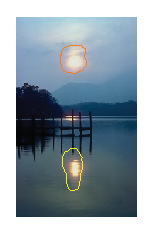
\includegraphics[height=0.28\textheight]{poisson_src1.eps}
	}
	\subfloat[Destination image]
	{
		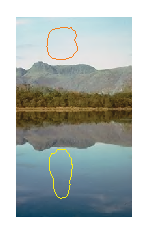
\includegraphics[height=0.28\textheight]{poisson_dest1.eps}
	}
	\subfloat[Cloning]
	{
		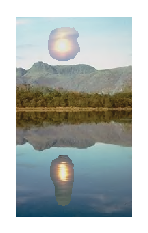
\includegraphics[height=0.28\textheight]{poisson_cloning1.eps}
	}
	\subfloat[Seamless cloning]
	{
		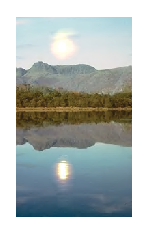
\includegraphics[height=0.28\textheight]{poisson_seamless_cloning1.eps}
	}
	\caption{First example of seamless cloning using Poisson image editing. All images in this figure are from the work of P{\'e}rez~\etal~\cite{Perez2003}.}
	\label{fig:seamless_cloning1}
\end{figure}
\begin{figure}
	\centering
	\parbox{\linewidth}
	{
		\parbox{0.3\linewidth}
		{
			\subfloat[Sources/destinations]
			{
				\begin{minipage}[t][5cm][t]{0.9\linewidth}
					\centering
					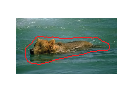
\includegraphics[height=0.05\textheight]{poisson_src2-1.eps}
					\vfill
					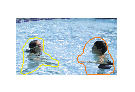
\includegraphics[height=0.05\textheight]{poisson_src2-2.eps}
					\vfill
					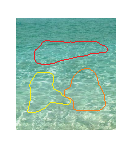
\includegraphics[height=0.15\textheight]{poisson_dest2.eps}
				\end{minipage}
			}
		}
		\hskip1em
		\parbox{0.3\linewidth}
		{
			\subfloat[Cloning]
			{
				\begin{minipage}[t][5cm][t]{0.9\linewidth}
					\centering
					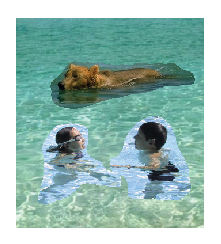
\includegraphics[width=0.9\linewidth]{poisson_cloning2.eps}
				\end{minipage}
			}
		}
		\hskip1em
		\parbox{0.3\linewidth}
		{
			\subfloat[Seamless cloning]
			{
				\begin{minipage}[t][5cm][t]{0.9\linewidth}
					\centering
					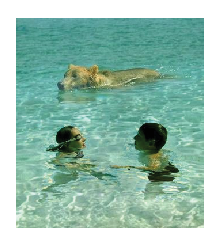
\includegraphics[width=0.9\linewidth]{poisson_seamless_cloning2.eps}
				\end{minipage}
			}
		}
	}
	\caption{Second example of seamless cloning using Poisson image edting. Unlike the first example, there are three regions from two source images for one destination image. All images in this figure are from the work of P{\'e}rez~\etal~\cite{Perez2003}.}
	\label{fig:seamless_cloning2}
\end{figure}
To make a condensed video, foregrounds of the rearranged object tubes are stitched with the background images by utilizing Poisson image editing~\cite{Perez2003}. What we can do with Poisson image editing is inserting some part of the source image to the destination image seamlessly as shown in \Cref{fig:seamless_cloning1} and \Cref{fig:seamless_cloning2}.

Before explaining the mathematics behind this editing, some notations need to be defined first. In \Cref{fig:poisson_notation}, $\boldsymbol{S}$ is a spatial domain of the destination image and belongs to $\mathbb{R}^2$, $\boldsymbol\Omega$ is the domain to be edited and has a boundary $\partial\boldsymbol\Omega$, $g$ and $f^{*}$ are scalar functions of source and destination images, respectively, $f$ is an unknown function, and $\textbf{v}$ is a gradient field which will be explained later. In addition, $f^{*}$ is defined over $S-(\boldsymbol\Omega-\partial\boldsymbol\Omega)$ and $f$ is defined over $\boldsymbol\Omega$; therefore, $\partial\boldsymbol\Omega$ indicates an overlapped region between $\boldsymbol{S}$ and $\boldsymbol\Omega$.

\begin{figure}
	\centering
	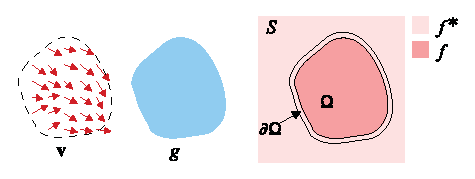
\includegraphics[width=0.9\linewidth]{poisson_image_editing_notation.eps}
	\caption{Notations used in Poisson image editing~\cite{Perez2003}.}
	\label{fig:poisson_notation}
\end{figure}
As you can see in \Cref{fig:poisson_notation}, the objective of the editing is to find a proper $f$ satisfying the boundary condition on $\boldsymbol\Omega$. One example of achieving the objective is minimizing the following equation.
\begin{equation}
\label{eq:min_field}
\min_f \iint_{\boldsymbol\Omega} |\nabla f - \textbf{v}|^2 \quad \textrm{with} \quad f|_{\boldsymbol\partial\Omega}=f^{*}|_{\boldsymbol\partial\Omega}.
\end{equation}
The unique solution of (\ref{eq:min_field}) can be obtained by solving following Poisson equation with Dirichlet boundary condition.
\begin{equation}
\label{eq:poisson}
\Delta f = \textrm{div}\textbf{v} \quad \textrm{over} \quad \boldsymbol\Omega \quad \textrm{with} \quad f|_{\boldsymbol\partial\Omega}=f^{*}|_{\boldsymbol\partial\Omega},
\end{equation}
where div$\cdot$ is a divergence operator; hence $\textrm{div}\textbf{v}= \left( \frac{\partial u}{\partial x},\frac{\partial v}{\partial y} \right)$, when $\textbf{v}=(u, v)$. In (\ref{eq:min_field}) and (\ref{eq:poisson}), $\textbf{v}$ is used as a guidance field; therefore, how to choose $\textbf{v}$ can change the purpose of the editing. One possible choice of $\textbf{v}$ to seamlessly insert one image to another is $\nabla g$. Then, (\ref{eq:poisson}) is changed to
\begin{equation}
\label{eq:poisson2}
\Delta f = \Delta g \quad \textrm{over} \quad \boldsymbol\Omega \quad \textrm{with} \quad f|_{\boldsymbol\partial\Omega}=f^{*}|_{\boldsymbol\partial\Omega}.
\end{equation}
The equation (\ref{eq:poisson2}) means that the Laplacian of the inserted region is identical to that of the source while pixel intensities of the destination over the inserted region's boundary remain unchanged.

\Cref{fig:poisson_fg_bg} shows example frames of the condensed video after applying either na\"ive alpha blending or Poisson image editing for the stitching process. As you can see in the figure, results using Poisson image editing are more visually natural but it takes more computation time than the na\"ive approach.
\begin{figure}
	\centering
	\caption{Figure will be inserted here.}
	\label{fig:poisson_fg_bg}
\end{figure}

\section{Discontinuity of motion flow}
\begin{figure}
	\centering
	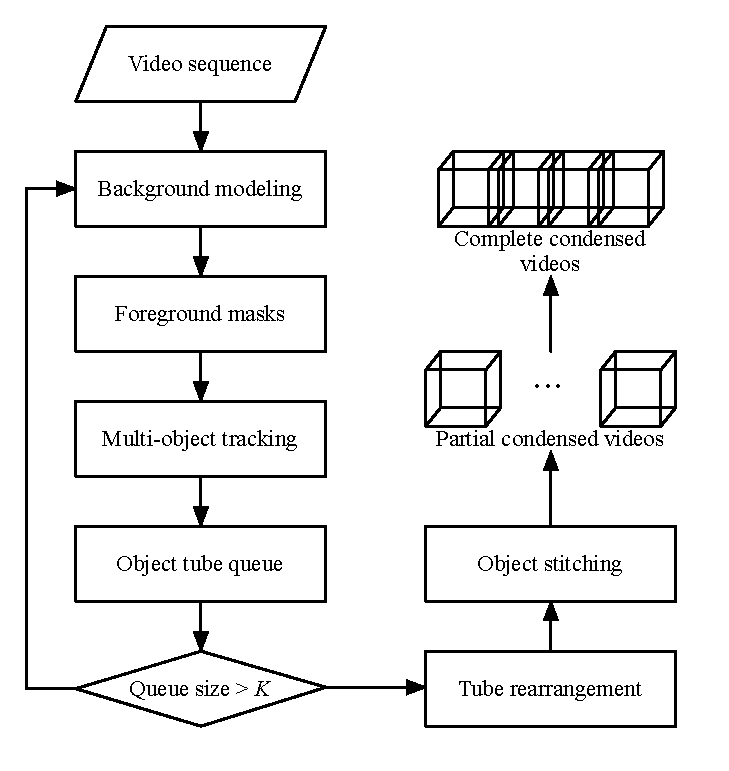
\includegraphics[width=0.8\linewidth]{framework.pdf}
	\caption{Proposed online video synopsis framework. The framework generates a partial condensed video whenever the size of the queue exceeds $K$. Then, partial videos are merged into the complete synopsis video.}
	\label{fig:framework}
\end{figure}
As shown in \Cref{fig:framework}, online video synopsis generates a small portion of the condensed video containing $K$ object tubes after each tube rearrangement step. If we have $20 \times K$ object tubes, there will be 20 portions of the condensed video. At the time of the user request, these portions are merged into the complete synopsis video. During the merging process, if we could not properly handle the transitions between the one portion to another, the users might notice the abrupt changes in the scene. This problem is called as a discontinuity of motion flow. One simple yet efficient way to prevent such discontinuity is considering tails of the object tubes in the previous iteration during the current step~\cite{Fu2014}. \Cref{fig:discontinuity} shows diagrams to explain the solution.
\begin{figure}
	\subfloat[Rearranged tubes after $1^{\rm{st}}$ iteration]
	{
		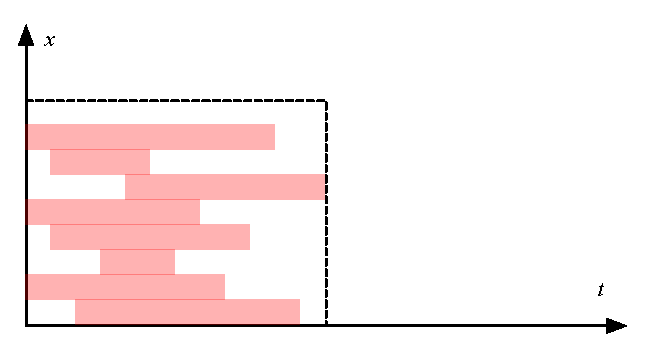
\includegraphics[width=0.9\linewidth]{discontinuity.pdf}
		\label{fig:discontinuity:1}
	}
	\\
	\subfloat[Rearranged tubes after $2^{\rm{nd}}$ iteration]
	{
		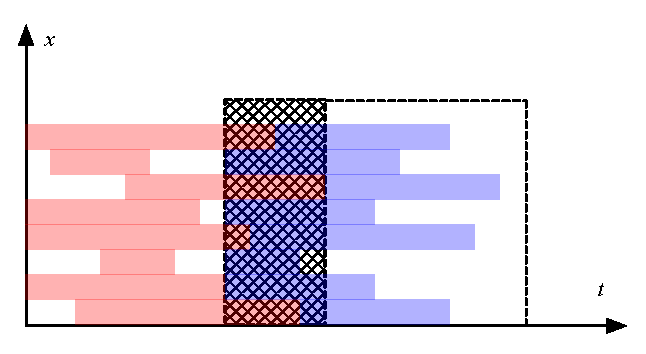
\includegraphics[width=0.9\linewidth]{discontinuity2.pdf}
		\label{fig:discontinuity:2}
	}
	\caption{Simple solution for the discontinuity of motion flow problem. When finding optimum starting labels for $2^{\rm{nd}}$ iteration, tails of the object tubes rearranged at $1^{\rm{st}}$ iteration (patterned region) are considered as obstacles as shown in \protect\subref{fig:discontinuity:2}.}
	\label{fig:discontinuity}
\end{figure}

\chapter{Experimental Results}
\label{sec:exp}

\section{Performance metrics}
In this chapter, the performance of the proposed tube rearrangement algorithm is evaluated by using four metrics: frame condensation ratio (FR), compact ratio (CR), overlap ratio (OR), and running time (RT). The detail of each performance metric is presented as follows.

FR is defined as a ratio of the condensed video length to the original video.
\begin{equation}
\textrm{FR} = \frac{\mathcal{T}^{*}}{\mathcal{T}},
\end{equation}
where $\mathcal{T}^{*}$ and $\mathcal{T}$ are lengths of the condensed and original videos, respectively. Smaller FR is better for reducing time consumption of browsing contents of the video.

CR indicates that how many pixels in the condensed video are occupied by the objects and is defined as
\begin{equation}
\label{eq:CR}
\textrm{CR}=\frac{1}{\mathcal{W}\mathcal{H}\mathcal{T}^{*}}\sum_{x=1}^{\mathcal{W}}\sum_{y=1}^{\mathcal{H}}\sum_{t=1}^{\mathcal{T}^{*}} F^{*}(x,y,t) = \frac{|F^{*}|}{\mathcal{W}\mathcal{H}\mathcal{T}^{*}},
\end{equation}
where $F^{*}$ is a foreground volume of the condensed video. Each element of $F^{*}$ is defined as
\begin{equation}
F^{*}(x,y,t)=
\begin{cases}
1 & I^{*}(x,y,t) \neq B_t(x,y,t)\\
0 & \rm{otherwise},
\end{cases}
\end{equation}
where $I^{*}(x,y,t)$ is a pixel of the condensed video and $B_t(x,y,t)$ is a pixel of the time-lapse background before the stitching process. A large CR indicates that the tube rearrangement algorithm effectively utilizes the spatio-temporal domain of the synopsis video.

OR is proportional to the number of overlapped foreground pixels in the condensed video and defined as
\begin{equation}
\textrm{OR}=\frac{1}{|F^{*}|}\sum_{x=1}^{\mathcal{W}}\sum_{y=1}^{\mathcal{H}}\sum_{t=1}^{\mathcal{T}^{*}} O(x,y,t)=\frac{|O|}{|F^{*}|},
\end{equation}
where $O(x,y,t)$ is activated to 1, when $I^{*}(x,y,t)$ is a result of blending foreground pixels of two or more objects with $B_t(x,y,t)$; otherwise, it produces 0. If OR is small, we can easily distinguish rearranged objects in the synopsis video; therefore, we can understand the summarized information better.

The last but not least RT is a metric to compare computational complexity of the algorithm and measured in seconds. This metric is important when the framework responds to the requests of users. Smaller RT is better for reducing a latency of the system. All experiments in following sections are conducted on a 4-core 4.0 GHz computer with 32 GB of memory. 

\section{Test video sequences}
For the test sequences, six video clips are captured at four different places: a parking lot square, a crossroad, a library lobby, and a subway station plaza. Detail characteristics of the test sequences are summarized in Table~\ref{tb:video_perf}. Some examples of the test sequences are depicted in \Cref{fig:examples}.

Parking lot square I sequence mainly focuses on the entrance of the parking lot but there is a sidewalk with red bricks on the left. Since this place is a main road to most of buildings in Hanyang university, the scene is very crowded with people. The scene of Parking lot square II is similar to that of Parking lot square I, but the most of moving objects are vehicle not pedestrian.

Crossroad I and II sequences are captured at the same place with different seasons and camera's zoom parameter. Crossroad I is captured at summer with more zoom, while Crossroad II is captured at fall with less zoom. Most of people appeared in this scene walk in either left or right directions.

Library lobby sequence is captured by the indoor security camera mounted on 2nd floor of the building. There is a gateway of the library at top of the scene and stairs (not visible in the scene) are located at left and right side of the building; therefore, people move from either left or right to the top, or vice versa.

Subway station plaza is an open place in front of the subway station entrance. Since there are many ways to get to the building from here, there is no dominant walking direction of people.

\begin{figure}
	\centering
	\subfloat[Parking lot square I]
	{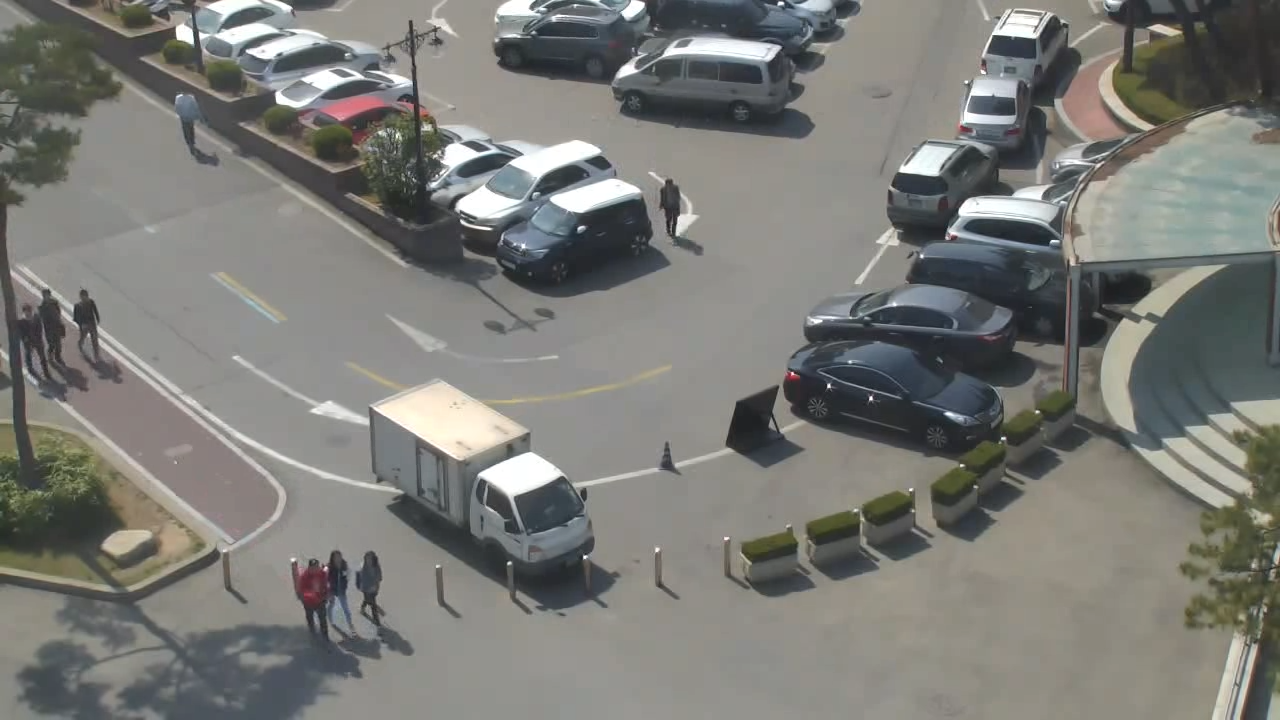
\includegraphics[width=0.45\linewidth]{fig/sidewalk.png}}
	\label{fig:sidewalk}
	\subfloat[Parking lot square II]
	{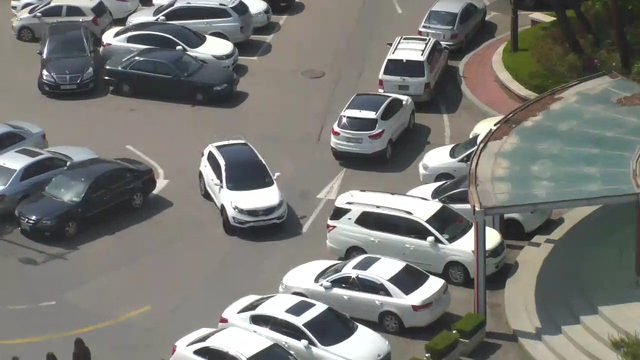
\includegraphics[width=0.45\linewidth]{fig/parking_lot.png}}
	\label{fig:crossroadI}
	\subfloat[Crossroad I]
	{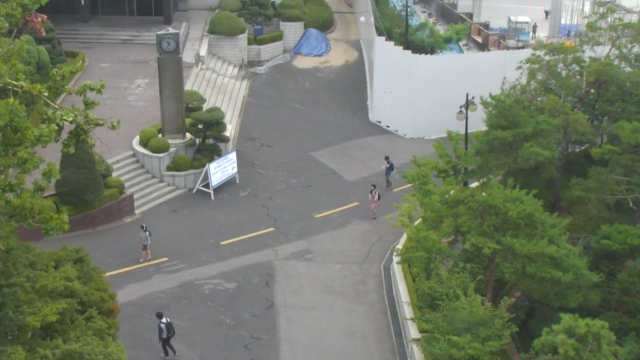
\includegraphics[width=0.45\linewidth]{fig/crossroad01.png}}
	\label{fig:crossroadII}
	\subfloat[Crossroad II]
	{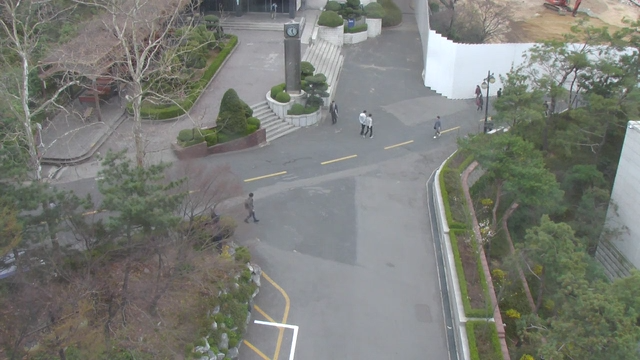
\includegraphics[width=0.45\linewidth]{fig/crossroad02.png}}
	\label{fig:library}
	\subfloat[Library lobby I]
	{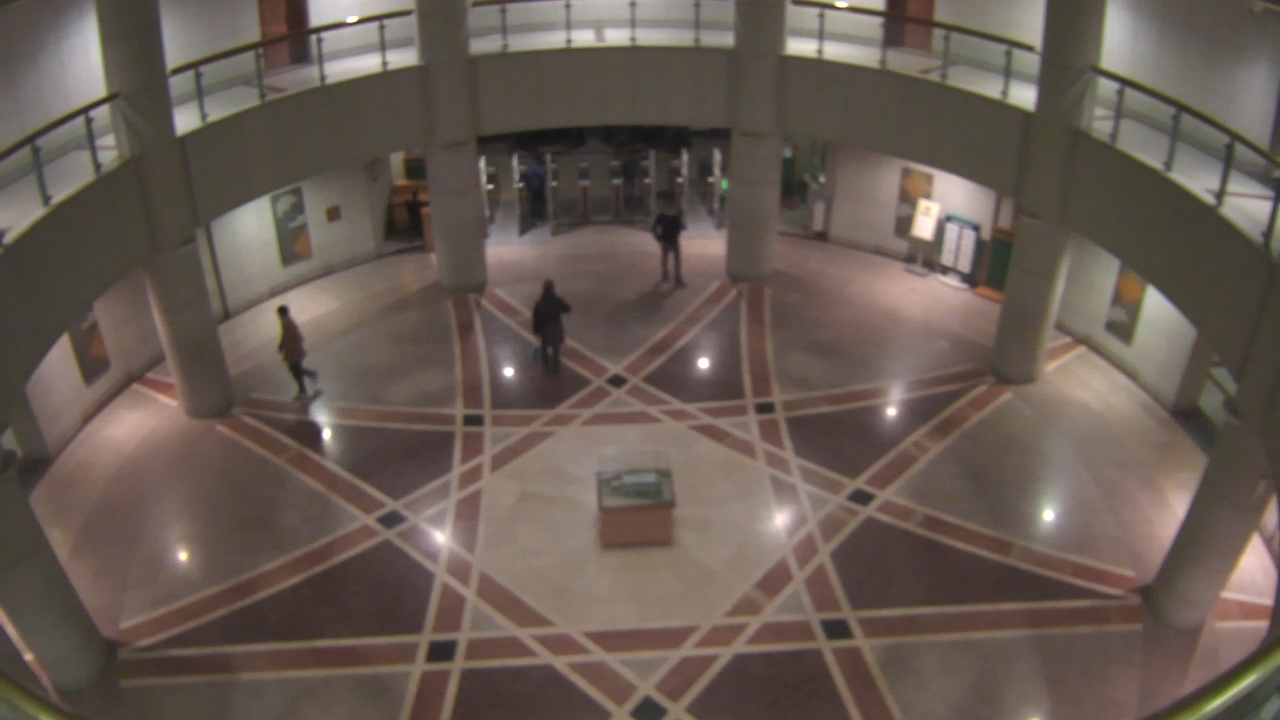
\includegraphics[width=0.45\linewidth]{fig/library.png}}
	\label{fig:parking_lot}
	\subfloat[Subway station plaza I]
	{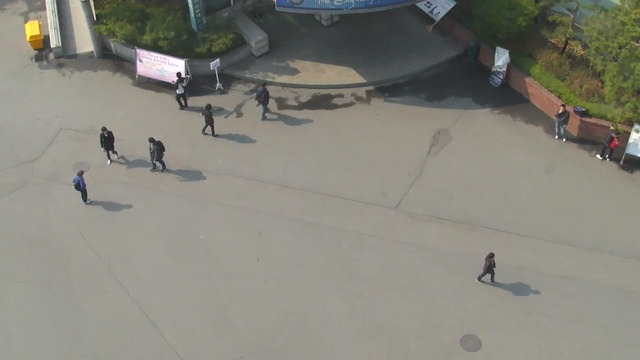
\includegraphics[width=0.45\linewidth]{fig/subway_entrance.png}}
	\label{fig:subway_entrance}
	\caption{Examples of the test sequences. All sequences were captured with three PTZ cameras at Hanyang university, Seoul, Korea.}
	\label{fig:examples}
\end{figure}
\begin{table}
	\begin{center}
		\begin{tabular}{clccc}
			\hline
			\hline
			Symbol & Video clip name & Resolution & \# Frame & \# Tube\\
			\hline
			\hline
			VC1 & Parking lot square I & $1280 \times 720$ & 44,057 & 650\\
			\hline
			VC2 & Parking lot square II & $640 \times 360$ & 107,946 & 271\\
			\hline
			VC3 & Crossroad I & $640 \times 360$ & 85,766 & 291\\
			\hline
			VC4 & Crossroad II & $640 \times 360$ & 106,459 & 937\\
			\hline
			VC5 & Library lobby I & $1280 \times 720$ & 49,679 & 316\\
			\hline
			VC6 & Subway station plaza I & $640 \times 360$ & 107,876 & 1038\\
			\hline
		\end{tabular}
	\end{center}
	\caption{List of test sequences used in the experiments.}
	\label{tb:video_perf}
\end{table}

\section{Performance analysis}
The experiments in this section are designed to 1) find optimum parameters for the proposed tube rearrangement algorithm, 2) conduct an ablation study for two speed up techniques, and 3) compare performances of several different online tube rearrangement algorithms.

\subsection{Optimum parameters}
\label{sec:exp:param}
There are four necessary parameters for the proposed tube rearrangement algorithm: the weight parameter of the length energy $\lambda$, the size of the occupation matrix $\mathcal{M}\times\mathcal{N}$, the type of the occupation matrix, and the size of the queue $K$. Apart from six test sequences used for the performance evaluation, additional five video clips are prepared to find optimum parameters and detail characteristics of the videos are summarized in Table~\ref{tb:video_param}.
\begin{table}
	\begin{center}
		\begin{tabular}{clccc}
			\hline
			\hline
			Symbol & Video clip name & Resolution & \# Frame & \# Tube\\
			\hline
			\hline
			VC7 & Crossroad III & $1280 \times 720$ & 106,558 & 831 \\
			\hline
			VC8 & Library lobby II & $1280 \times 720$ & 108,091 & 3,166 \\
			\hline
			VC9 & Subway station plaza II & $1280 \times 720$ & 134,622 & 2,311 \\
			\hline
			VC10 & Subway station plaza III & $1280 \times 720$ & 108,016 & 2,048 \\
			\hline
			VC11 & Subway station plaza IV & $1280 \times 720$ & 108,012 & 1,988 \\
			\hline
		\end{tabular}
	\end{center}
	\caption{List of sequences used to find optimum parameters of the proposed tube rearrangement algorithm.}
	\label{tb:video_param}
\end{table}

\subsubsection{Weight parameter of length energy}
\label{sec:exp:weight}
First experiment measures the four performance metrics by changing $\lambda$ from 1 to 5000. Remaining parameters are fixed as $\mathcal{M}\times\mathcal{N}=9\times16$, $K=20$, and the algorithm produces results for both binary and probabilistic occupation matrices. Except for RT, other three metrics have similar scales; hence, FR, CR and OR are depicted together in \Cref{fig:exp:lambda}. On the other hand, RT for five sequences are grouped and summarized in \Cref{fig:exp:lambda:RT}. 

As expected, FR decreases when the proposed algorithm pays more attention to the length energy (increasing $\lambda$). On the other hand, CR and OR do not change as much as FR. As shown in \Cref{fig:exp:lambda:RT}, we can see that RT is proportional to the number of object tubes in the original video, and tends to decrease as $\lambda$ increases. This result is quite obvious, because small number of object tubes and less frames to consider reduce the computational burden.

One interesting result is shown in \Cref{fig:exp:lambda:b}, where FR is larger than 1 for $\lambda \in \{1, 10, 50\}$ with binary occupation matrix and $\lambda=1$ with probabilistic occupation matrix. This result is induced by two factors: small $\lambda$ and large number of object tubes having similar paths. When $\lambda$ is small, the proposed algorithm focuses on reducing collisions rather than making a short length video. In addition, when large number of objects share the common path in the scene, it is hard to avoid collisions between the objects moving along the path. One straightforward solution for the rearrangement problem under these conditions is minimizing the overlapped time region between the objects. In other words, the algorithm rearranges object tubes like linked sausages and the resulting video may have a longer length than the original one. To avoid such undesirable solution, selecting sufficiently large $\lambda$ is important for the proposed algorithm. However, when $\lambda$ exceeds some value, four metrics become saturated, which means that the algorithm primarily considers the length energy. This solution is not desirable neither; therefore, we need to choose a balanced value of $\lambda$.

For selecting the value of $\lambda$, different behaviors of the binary and probabilistic occupation matrices should be considered. As you can see in \Cref{fig:exp:lambda,fig:exp:lambda:RT}, when $K$ increases, the algorithm utilizing the probabilistic occupation matrix approaches to the saturation point faster than the one using the binary occupation matrix. Therefore, with same $\lambda$, the probabilistic occupation matrix allows the algorithm to produce the shorter synopsis video than the binary occupation matrix; it other words, it has better FR and CR, but higher OR than its counterpart. Based on the observation, it is better to select different $\lambda$ for the probabilistic and binary occupation matrices. However, for easier parameter analysis in following sections, both types of the occupation matrix utilize $\lambda$ of 100.

\pgfplotstableread[col sep=comma]{exp_bin_occ/crossroad03_length_param.csv}\tableLambdaOne
\pgfplotstableread[col sep=comma]{exp_bin_occ/library02_length_param.csv}\tableLambdaTwo
\pgfplotstableread[col sep=comma]{exp_bin_occ/subway_entrance02_length_param.csv}\tableLambdaThree
\pgfplotstableread[col sep=comma]{exp_bin_occ/subway_entrance03_length_param.csv}\tableLambdaFour
\pgfplotstableread[col sep=comma]{exp_bin_occ/subway_entrance04_length_param.csv}\tableLambdaFive

\pgfplotstableread[col sep=comma]{exp_prob_occ/crossroad03_length_param.csv}\tableProbLambdaOne
\pgfplotstableread[col sep=comma]{exp_prob_occ/library02_length_param.csv}\tableProbLambdaTwo
\pgfplotstableread[col sep=comma]{exp_prob_occ/subway_entrance02_length_param.csv}\tableProbLambdaThree
\pgfplotstableread[col sep=comma]{exp_prob_occ/subway_entrance03_length_param.csv}\tableProbLambdaFour
\pgfplotstableread[col sep=comma]{exp_prob_occ/subway_entrance04_length_param.csv}\tableProbLambdaFive

\begin{figure}
	\centering
	\subfloat[Crossroad III]
	{
		\begin{tikzpicture}[scale = 1.0]
		\begin{axis}[
		xlabel = {$\lambda$},
		xtick = data,
		xticklabels from table = {\tableLambdaOne}{Domain},
		legend pos = outer north east,
		grid = major,
		]
		
		\addplot table [x expr=\coordindex, y=FR] {\tableLambdaOne};
		\addlegendentry{Bin-FR}
		\addplot table [x expr=\coordindex, y=CR] {\tableLambdaOne};
		\addlegendentry{Bin-CR}
		\addplot table [x expr=\coordindex, y=OR] {\tableLambdaOne};
		\addlegendentry{Bin-OR}
		\addplot table [x expr=\coordindex, y=FR] {\tableProbLambdaOne};
		\addlegendentry{Prob-FR}
		\addplot table [x expr=\coordindex, y=CR] {\tableProbLambdaOne};
		\addlegendentry{Prob-CR}
		\addplot table [x expr=\coordindex, y=OR] {\tableProbLambdaOne};
		\addlegendentry{Prob-OR}
		
		\end{axis}
		\end{tikzpicture}
	}
	\\
	\subfloat[Library lobby II]
	{
		\label{fig:exp:lambda:b}
		\begin{tikzpicture}[scale = 1.0]
		\begin{axis}[
		xlabel = {$\lambda$},
		xtick = data,
		xticklabels from table = {\tableLambdaTwo}{Domain},
		legend pos = outer north east,
		grid = major,
		]
		
		\addplot table [x expr=\coordindex, y=FR] {\tableLambdaTwo};
		\addlegendentry{Bin-FR}
		\addplot table [x expr=\coordindex, y=CR] {\tableLambdaTwo};
		\addlegendentry{Bin-CR}
		\addplot table [x expr=\coordindex, y=OR] {\tableLambdaTwo};
		\addlegendentry{Bin-OR}
		\addplot table [x expr=\coordindex, y=FR] {\tableProbLambdaTwo};
		\addlegendentry{Prob-FR}
		\addplot table [x expr=\coordindex, y=CR] {\tableProbLambdaTwo};
		\addlegendentry{Prob-CR}
		\addplot table [x expr=\coordindex, y=OR] {\tableProbLambdaTwo};
		\addlegendentry{Prob-OR}
		
		\end{axis}
		\end{tikzpicture}
	}
	\caption{Result of the experiment conducted by changing $\lambda$.}
	\label{fig:exp:lambda}
\end{figure}
\begin{figure}\ContinuedFloat
	\centering
	\subfloat[Subway station plaza II]
	{
		\begin{tikzpicture}[scale = 1.0]
		\begin{axis}[
		xlabel = {$\lambda$},
		xtick = data,
		xticklabels from table = {\tableLambdaThree}{Domain},
		legend pos = outer north east,
		grid = major,
		]
		
		\addplot table [x expr=\coordindex, y=FR] {\tableLambdaThree};
		\addlegendentry{Bin-FR}
		\addplot table [x expr=\coordindex, y=CR] {\tableLambdaThree};
		\addlegendentry{Bin-CR}
		\addplot table [x expr=\coordindex, y=OR] {\tableLambdaThree};
		\addlegendentry{Bin-OR}
		\addplot table [x expr=\coordindex, y=FR] {\tableProbLambdaThree};
		\addlegendentry{Prob-FR}
		\addplot table [x expr=\coordindex, y=CR] {\tableProbLambdaThree};
		\addlegendentry{Prob-CR}
		\addplot table [x expr=\coordindex, y=OR] {\tableProbLambdaThree};
		\addlegendentry{Prob-OR}
		
		\end{axis}
		\end{tikzpicture}
	}
	\\
	\subfloat[Subway station plaza III]
	{
		\begin{tikzpicture}[scale = 1.0]
		\begin{axis}[
		xlabel = {$\lambda$},
		xtick = data,
		xticklabels from table = {\tableLambdaFour}{Domain},
		legend pos = outer north east,
		grid = major,
		]
		
		\addplot table [x expr=\coordindex, y=FR] {\tableLambdaFour};
		\addlegendentry{Bin-FR}
		\addplot table [x expr=\coordindex, y=CR] {\tableLambdaFour};
		\addlegendentry{Bin-CR}
		\addplot table [x expr=\coordindex, y=OR] {\tableLambdaFour};
		\addlegendentry{Bin-OR}
		\addplot table [x expr=\coordindex, y=FR] {\tableProbLambdaFour};
		\addlegendentry{Prob-FR}
		\addplot table [x expr=\coordindex, y=CR] {\tableProbLambdaFour};
		\addlegendentry{Prob-CR}
		\addplot table [x expr=\coordindex, y=OR] {\tableProbLambdaFour};
		\addlegendentry{Prob-OR}
		
		\end{axis}
		\end{tikzpicture}
	}
	\caption{(continued) Result of the experiment conducted by changing $\lambda$.}
\end{figure}
\begin{figure}\ContinuedFloat
	\centering
	\subfloat[Subway station plaza IV]
	{
		\begin{tikzpicture}[scale = 1.0]
		\begin{axis}[
		xlabel = {$\lambda$},
		xtick = data,
		xticklabels from table = {\tableLambdaFive}{Domain},
		legend pos = outer north east,
		grid = major,
		]
		
		\addplot table [x expr=\coordindex, y=FR] {\tableLambdaFive};
		\addlegendentry{Bin-FR}
		\addplot table [x expr=\coordindex, y=CR] {\tableLambdaFive};
		\addlegendentry{Bin-CR}
		\addplot table [x expr=\coordindex, y=OR] {\tableLambdaFive};
		\addlegendentry{Bin-OR}
		\addplot table [x expr=\coordindex, y=FR] {\tableProbLambdaFive};
		\addlegendentry{Prob-FR}
		\addplot table [x expr=\coordindex, y=CR] {\tableProbLambdaFive};
		\addlegendentry{Prob-CR}
		\addplot table [x expr=\coordindex, y=OR] {\tableProbLambdaFive};
		\addlegendentry{Prob-OR}
		
		\end{axis}
		\end{tikzpicture}
	}
	\caption{(continued) Result of the experiment conducted by changing $\lambda$.}
\end{figure}
\begin{sidewaysfigure}
	\centering
	\subfloat[Binary occupation matrix]
	{
		\begin{tikzpicture}[scale = 1.0]
		\begin{axis}[
		title = {Running time},
		xlabel = {$\lambda$},
		ylabel = {Seconds},
		ymax = 5,
		xtick = data,
		xticklabels from table = {\tableLambdaOne}{Domain},
		grid = major,
		]
		
		\addplot table [x expr=\coordindex, y=RT] {\tableLambdaOne};
		\addplot table [x expr=\coordindex, y=RT] {\tableLambdaTwo};
		\addplot table [x expr=\coordindex, y=RT] {\tableLambdaThree};
		\addplot table [x expr=\coordindex, y=RT] {\tableLambdaFour};
		\addplot table [x expr=\coordindex, y=RT] {\tableLambdaFive};
		
		\end{axis}
		\end{tikzpicture}
	}
	\subfloat[Probabilistic occupation matrix]
	{
		\begin{tikzpicture}[scale = 1.0]
		\begin{axis}[
		title = {Running time},
		xlabel = {$\lambda$},
		ymax = 5,
		xtick = data,
		xticklabels from table = {\tableLambdaOne}{Domain},
		legend pos = outer north east,
		grid = major,
		]
		
		\addplot table [x expr=\coordindex, y=RT] {\tableProbLambdaOne};
		\addlegendentry{VC7}
		\addplot table [x expr=\coordindex, y=RT] {\tableProbLambdaTwo};
		\addlegendentry{VC8}
		\addplot table [x expr=\coordindex, y=RT] {\tableProbLambdaThree};
		\addlegendentry{VC9}
		\addplot table [x expr=\coordindex, y=RT] {\tableProbLambdaFour};
		\addlegendentry{VC10}
		\addplot table [x expr=\coordindex, y=RT] {\tableProbLambdaFive};
		\addlegendentry{VC11}
		
		\end{axis}
		\end{tikzpicture}
	}
	\caption{RT of the proposed algorithm measured by changing $\lambda$ for five sequences.}
	\label{fig:exp:lambda:RT}
\end{sidewaysfigure}

\subsubsection{Size of occupation matrix}
\label{sec:exp:occ}
Second experiment is conducted by changing spatial resolution $\mathcal{M}\times\mathcal{N}$ of the occupation matrix. Assume that the aspect ratio of the input video is 16:9 (the ratio of the width to the height). Based on the assumption, four candidates of $\mathcal{M}\times\mathcal{N}$ are considered in this experiment: $9\times16$, $18\times32$, $36\times64$, and $72\times128$. Remaining parameters are fixed as $\lambda=100$ and $K=20$ and the algorithm utilizes both binary and probabilistic occupation matrices.

The larger binary occupation matrix has a better ability to encode the locations of the objects; therefore, the algorithm can finely adjust starting labels to avoid collisions. Then, the resulting video has lower FR and higher CR than the one using the smaller occupation matrix as shown in \Cref{fig:exp:occ}. However, interestingly, increasing the resolution of the probabilistic occupation matrix does not affect to the performance regarding three metrics. This indicates that even the low resolution probabilistic occupation matrix has already got enough capability to express fine locations of the objects.

In terms of RT, reducing spatial resolution for both types of the occupation matrix drastically increases the computation speed of the algorithm as depicted in \Cref{fig:exp:occ:RT}. According to \Cref{tb:exp:occ:RT}, in overall, the probabilistic occupation matrix can compute rearranged starting labels faster than the binary occupation matrix; however, the tendency of the computation time for different $\mathcal{M}\times\mathcal{N}$ is almost identical. Especially, the computation time for both types of the occupation matrix is reduced by at least 1/40, when the width and height of the matrix are scaled by 1/8 (from $72\times128$ to $9\times16$).

In summary, there are definite advantages in FR and CR for increasing the spatial resolution of the binary matrix; however, the degradation of the computation speed is too serious to be neglected. On the other hand, large probabilistic occupation matrix does not have any advantages regarding the performance metrics, and even with the low resolution matrix, the algorithm can have a better condensation ability than the one uses the high resolution binary matrix. Therefore, for both types of the occupation matrix, the smallest resolution ($9\times16$) is preferred in this dissertation.

\pgfplotstableread[col sep=comma]{exp_bin_occ/crossroad03_size_of_occupation_matrix.csv}\tableOccSzOne
\pgfplotstableread[col sep=comma]{exp_bin_occ/library02_size_of_occupation_matrix.csv}\tableOccSzTwo
\pgfplotstableread[col sep=comma]{exp_bin_occ/subway_entrance02_size_of_occupation_matrix.csv}\tableOccSzThree
\pgfplotstableread[col sep=comma]{exp_bin_occ/subway_entrance03_size_of_occupation_matrix.csv}\tableOccSzFour
\pgfplotstableread[col sep=comma]{exp_bin_occ/subway_entrance04_size_of_occupation_matrix.csv}\tableOccSzFive

\pgfplotstableread[col sep=comma]{exp_prob_occ/crossroad03_size_of_occupation_matrix.csv}\tableProbOccSzOne
\pgfplotstableread[col sep=comma]{exp_prob_occ/library02_size_of_occupation_matrix.csv}\tableProbOccSzTwo
\pgfplotstableread[col sep=comma]{exp_prob_occ/subway_entrance02_size_of_occupation_matrix.csv}\tableProbOccSzThree
\pgfplotstableread[col sep=comma]{exp_prob_occ/subway_entrance03_size_of_occupation_matrix.csv}\tableProbOccSzFour
\pgfplotstableread[col sep=comma]{exp_prob_occ/subway_entrance04_size_of_occupation_matrix.csv}\tableProbOccSzFive

\begin{figure}
	\centering
	\subfloat[Crossroad III]
	{
		\begin{tikzpicture}[scale = 1.0]
		\begin{axis}[
		xlabel = {$\mathcal{M}\times\mathcal{N}$},
		xtick = data,
		xticklabels from table = {\tableOccSzOne}{Domain},
		legend pos = outer north east,
		grid = major,
		]
		
		\addplot table [x expr=\coordindex, y=FR] {\tableOccSzOne};
		\addlegendentry{Bin-FR}
		\addplot table [x expr=\coordindex, y=CR] {\tableOccSzOne};
		\addlegendentry{Bin-CR}
		\addplot table [x expr=\coordindex, y=OR] {\tableOccSzOne};
		\addlegendentry{Bin-OR}
		\addplot table [x expr=\coordindex, y=FR] {\tableProbOccSzOne};
		\addlegendentry{Prob-FR}
		\addplot table [x expr=\coordindex, y=CR] {\tableProbOccSzOne};
		\addlegendentry{Prob-CR}
		\addplot table [x expr=\coordindex, y=OR] {\tableProbOccSzOne};
		\addlegendentry{Prob-OR}
		
		\end{axis}
		\end{tikzpicture}
	}
	\\
	\subfloat[Library lobby II]
	{
		\begin{tikzpicture}[scale = 1.0]
		\begin{axis}[
		xlabel = {$\mathcal{M}\times\mathcal{N}$},
		xtick = data,
		xticklabels from table = {\tableOccSzTwo}{Domain},
		legend pos = outer north east,
		grid = major,
		]
		
		\addplot table [x expr=\coordindex, y=FR] {\tableOccSzTwo};
		\addlegendentry{Bin-FR}
		\addplot table [x expr=\coordindex, y=CR] {\tableOccSzTwo};
		\addlegendentry{Bin-CR}
		\addplot table [x expr=\coordindex, y=OR] {\tableOccSzTwo};
		\addlegendentry{Bin-OR}
		\addplot table [x expr=\coordindex, y=FR] {\tableProbOccSzTwo};
		\addlegendentry{Prob-FR}
		\addplot table [x expr=\coordindex, y=CR] {\tableProbOccSzTwo};
		\addlegendentry{Prob-CR}
		\addplot table [x expr=\coordindex, y=OR] {\tableProbOccSzTwo};
		\addlegendentry{Prob-OR}
		
		\end{axis}
		\end{tikzpicture}
	}
	\caption{Result of the experiment conducted by changing $\mathcal{M}\times\mathcal{N}$.}
	\label{fig:exp:occ}
\end{figure}
\begin{figure}\ContinuedFloat
	\centering
	\subfloat[Subway station plaza II]
	{
		
		\begin{tikzpicture}[scale = 1.0]
		\begin{axis}[
		xlabel = {$\mathcal{M}\times\mathcal{N}$},
		xtick = data,
		xticklabels from table = {\tableOccSzThree}{Domain},
		legend pos = outer north east,
		grid = major,
		]
		
		\addplot table [x expr=\coordindex, y=FR] {\tableOccSzThree};
		\addlegendentry{Bin-FR}
		\addplot table [x expr=\coordindex, y=CR] {\tableOccSzThree};
		\addlegendentry{Bin-CR}
		\addplot table [x expr=\coordindex, y=OR] {\tableOccSzThree};
		\addlegendentry{Bin-OR}
		\addplot table [x expr=\coordindex, y=FR] {\tableProbOccSzThree};
		\addlegendentry{Prob-FR}
		\addplot table [x expr=\coordindex, y=CR] {\tableProbOccSzThree};
		\addlegendentry{Prob-CR}
		\addplot table [x expr=\coordindex, y=OR] {\tableProbOccSzThree};
		\addlegendentry{Prob-OR}
		
		\end{axis}
		\end{tikzpicture}
	}
	\\
	\subfloat[Subway station plaza III]
	{
		\begin{tikzpicture}[scale = 1.0]
		\begin{axis}[
		xlabel = {$\mathcal{M}\times\mathcal{N}$},
		xtick = data,
		xticklabels from table = {\tableOccSzFour}{Domain},
		legend pos = outer north east,
		grid = major,
		]
		
		\addplot table [x expr=\coordindex, y=FR] {\tableOccSzFour};
		\addlegendentry{Bin-FR}
		\addplot table [x expr=\coordindex, y=CR] {\tableOccSzFour};
		\addlegendentry{Bin-CR}
		\addplot table [x expr=\coordindex, y=OR] {\tableOccSzFour};
		\addlegendentry{Bin-OR}
		\addplot table [x expr=\coordindex, y=FR] {\tableProbOccSzFour};
		\addlegendentry{Prob-FR}
		\addplot table [x expr=\coordindex, y=CR] {\tableProbOccSzFour};
		\addlegendentry{Prob-CR}
		\addplot table [x expr=\coordindex, y=OR] {\tableProbOccSzFour};
		\addlegendentry{Prob-OR}
		
		\end{axis}
		\end{tikzpicture}
	}
	\caption{(continued) Result of the experiment conducted by changing $\mathcal{M}\times\mathcal{N}$.}
\end{figure}
\begin{figure}\ContinuedFloat
	\centering
	\subfloat[Subway station plaza IV]
	{
		\begin{tikzpicture}[scale = 1.0]
		\begin{axis}[
		xlabel = {$\mathcal{M}\times\mathcal{N}$},
		xtick = data,
		xticklabels from table = {\tableOccSzFive}{Domain},
		legend pos = outer north east,
		grid = major,
		]
		
		\addplot table [x expr=\coordindex, y=FR] {\tableOccSzFive};
		\addlegendentry{Bin-FR}
		\addplot table [x expr=\coordindex, y=CR] {\tableOccSzFive};
		\addlegendentry{Bin-CR}
		\addplot table [x expr=\coordindex, y=OR] {\tableOccSzFive};
		\addlegendentry{Bin-OR}
		\addplot table [x expr=\coordindex, y=FR] {\tableProbOccSzFive};
		\addlegendentry{Prob-FR}
		\addplot table [x expr=\coordindex, y=CR] {\tableProbOccSzFive};
		\addlegendentry{Prob-CR}
		\addplot table [x expr=\coordindex, y=OR] {\tableProbOccSzFive};
		\addlegendentry{Prob-OR}
		
		\end{axis}
		\end{tikzpicture}
	}
	\caption{(continued) Result of the experiment conducted by changing $\mathcal{M}\times\mathcal{N}$.}
\end{figure}
\begin{sidewaysfigure}
	\centering
	\subfloat[Binary occupation matrix]
	{
		\begin{tikzpicture}[scale = 1.0]
		\begin{axis}[
		title = {Running time},
		xlabel = {$\mathcal{M}\times\mathcal{N}$},
		ylabel = {Seconds},
		ymax = 160,
		xtick = data,
		xticklabels from table = {\tableOccSzOne}{Domain},
		legend pos = outer north east,
		grid = major,
		]
		
		\addplot table [x expr=\coordindex, y=RT] {\tableOccSzOne};
		\addplot table [x expr=\coordindex, y=RT] {\tableOccSzTwo};
		\addplot table [x expr=\coordindex, y=RT] {\tableOccSzThree};
		\addplot table [x expr=\coordindex, y=RT] {\tableOccSzFour};
		\addplot table [x expr=\coordindex, y=RT] {\tableOccSzFive};
		
		\end{axis}
		\end{tikzpicture}
	}
	\subfloat[Probabilistic occupation matrix]
	{
		\begin{tikzpicture}[scale = 1.0]
		\begin{axis}[
		title = {Running time},
		xlabel = {$\mathcal{M}\times\mathcal{N}$},
		xtick = data,
		ymax = 160,
		xticklabels from table = {\tableOccSzOne}{Domain},
		legend pos = outer north east,
		grid = major,
		]
		
		\addplot table [x expr=\coordindex, y=RT] {\tableProbOccSzOne};
		\addlegendentry{VC7}
		\addplot table [x expr=\coordindex, y=RT] {\tableProbOccSzTwo};
		\addlegendentry{VC8}
		\addplot table [x expr=\coordindex, y=RT] {\tableProbOccSzThree};
		\addlegendentry{VC9}
		\addplot table [x expr=\coordindex, y=RT] {\tableProbOccSzFour};
		\addlegendentry{VC10}
		\addplot table [x expr=\coordindex, y=RT] {\tableProbOccSzFive};
		\addlegendentry{VC11}
		
		\end{axis}
		\end{tikzpicture}
	}
	\caption{RT of the proposed algorithm measured by changing $\mathcal{M}\times\mathcal{N}$ for five sequences.}
	\label{fig:exp:occ:RT}
\end{sidewaysfigure}

\pgfplotstableset{
	create on use/Domain/.style={
		create col/set list={$9\times16$,$18\times32$,$36\times64$,$64\times128$}},
}
\pgfplotstablenew[columns={Domain}]{4}\tableOccSzRT
\pgfplotstablecreatecol[copy column from table={\tableOccSzOne}{RT}]{VC7Bin}{\tableOccSzRT}
\pgfplotstablecreatecol[copy column from table={\tableProbOccSzOne}{RT}]{VC7Prob}{\tableOccSzRT}
\pgfplotstablecreatecol[copy column from table={\tableOccSzTwo}{RT}]{VC8Bin}{\tableOccSzRT}
\pgfplotstablecreatecol[copy column from table={\tableProbOccSzTwo}{RT}]{VC8Prob}{\tableOccSzRT}
\pgfplotstablecreatecol[copy column from table={\tableOccSzThree}{RT}]{VC9Bin}{\tableOccSzRT}
\pgfplotstablecreatecol[copy column from table={\tableProbOccSzThree}{RT}]{VC9Prob}{\tableOccSzRT}
\pgfplotstablecreatecol[copy column from table={\tableOccSzFour}{RT}]{VC10Bin}{\tableOccSzRT}
\pgfplotstablecreatecol[copy column from table={\tableProbOccSzFour}{RT}]{VC10Prob}{\tableOccSzRT}
\pgfplotstablecreatecol[copy column from table={\tableOccSzFive}{RT}]{VC11Bin}{\tableOccSzRT}
\pgfplotstablecreatecol[copy column from table={\tableProbOccSzFive}{RT}]{VC11Prob}{\tableOccSzRT}
\begin{sidewaystable}
	\centering
	\pgfplotstabletypeset[
	every first column/.style={string type, column name={}},
	every head row/.style={
		before row={
			\toprule
			& \multicolumn{2}{c}{VC7} & \multicolumn{2}{c}{VC8} & \multicolumn{2}{c}{VC9} & \multicolumn{2}{c}{VC10} & \multicolumn{2}{c}{VC11}\\
		},
		after row=\midrule,
	},
	every last row/.style={
		after row=\bottomrule},
	columns/VC7Bin/.style={column name=Bin.},
	columns/VC8Bin/.style={column name=Bin.},
	columns/VC9Bin/.style={column name=Bin.},
	columns/VC10Bin/.style={column name=Bin.},
	columns/VC11Bin/.style={column name=Bin.},
	columns/VC7Prob/.style={column name=Prob.},
	columns/VC8Prob/.style={column name=Prob.},
	columns/VC9Prob/.style={column name=Prob.},
	columns/VC10Prob/.style={column name=Prob.},
	columns/VC11Prob/.style={column name=Prob.},
	]{\tableOccSzRT}
	\caption{RT of the proposed algorithm measured in seconds by changing $\mathcal{M}\times\mathcal{N}$ for five video clips.}
	\label{tb:exp:occ:RT}
\end{sidewaystable}

\subsubsection{Size of queue}
\label{sec:exp:queue}
Adjusting the size of the queue $K$ determines how many object tubes are considered during each tube rearrangement step. The experiment is conducted as same manner as in \Cref{sec:exp:weight,sec:exp:occ}, while $K$ is changed from 10 to 100 with 10 interval. Other parameters are fixed to $\lambda=100$ and $\mathcal{M}\times\mathcal{N}=9\times16$, and both binary and probabilistic occupation matrix are used as spatial approximations of the foreground pixels. Results of the experiments are presented in \Cref{fig:exp:queue,fig:exp:queue:RT}.

For the binary occupation matrix, \Cref{fig:exp:queue} shows that, for increasing $K$, FR is decreased by at least 0.2 and CR is slightly increased, while OR remains almost unchanged. On the other hand, in general, the algorithm using the probabilistic matrix produces shorter synopsis videos with higher CR and OR. The key difference between the binary and occupation matrices is that the algorithm using the binary matrix produces synopsis videos having constant OR regardless of $K$. In other words, the resulting synopsis video never becomes more crowded even if $K$ is large.

It is obvious that the algorithm takes more time to get rearranged labels for increasing $K$ as shown in \Cref{fig:exp:queue:RT}. Additionally, the computational advantage of the probabilistic matrix over the binary matrix is clearly seen in the result. As discussed many times throughout \Cref{sec:exp:param}, since the algorithm using the probabilistic matrix produces shorter synopsis videos than the one using the binary matrix, the number of frames to consider during the tube rearrangement stage becomes smaller. In consequence, slopes of \Cref{fig:exp:queue:RT:b} are less steeper than that of \Cref{fig:exp:queue:RT:a}.

Similar to selecting $\lambda$, there is a trade-off between RT and other metrics for selecting $K$. Empirically, for both binary and probabilistic matrices, a median of the candidate values, 50, is used throughout the subsequent experiments.

\pgfplotstableread[col sep=comma]{exp_bin_occ/crossroad03_size_of_queue.csv}\tableQueueOne
\pgfplotstableread[col sep=comma]{exp_bin_occ/library02_size_of_queue.csv}\tableQueueTwo
\pgfplotstableread[col sep=comma]{exp_bin_occ/subway_entrance02_size_of_queue.csv}\tableQueueThree
\pgfplotstableread[col sep=comma]{exp_bin_occ/subway_entrance03_size_of_queue.csv}\tableQueueFour
\pgfplotstableread[col sep=comma]{exp_bin_occ/subway_entrance04_size_of_queue.csv}\tableQueueFive

\pgfplotstableread[col sep=comma]{exp_prob_occ/crossroad03_size_of_queue.csv}\tableProbQueueOne
\pgfplotstableread[col sep=comma]{exp_prob_occ/library02_size_of_queue.csv}\tableProbQueueTwo
\pgfplotstableread[col sep=comma]{exp_prob_occ/subway_entrance02_size_of_queue.csv}\tableProbQueueThree
\pgfplotstableread[col sep=comma]{exp_prob_occ/subway_entrance03_size_of_queue.csv}\tableProbQueueFour
\pgfplotstableread[col sep=comma]{exp_prob_occ/subway_entrance04_size_of_queue.csv}\tableProbQueueFive

\begin{figure}
	\centering
	\subfloat[Crossroad III]
	{
		\begin{tikzpicture}[scale = 1.0]
		\begin{axis}[
		xlabel = {$K$},
		xtick = data,
		xticklabels from table = {\tableQueueOne}{Domain},
		legend pos = outer north east,
		grid = major,
		]
		
		\addplot table [x expr=\coordindex, y=FR] {\tableQueueOne};
		\addlegendentry{Bin-FR}
		\addplot table [x expr=\coordindex, y=CR] {\tableQueueOne};
		\addlegendentry{Bin-CR}
		\addplot table [x expr=\coordindex, y=OR] {\tableQueueOne};
		\addlegendentry{Bin-OR}
		\addplot table [x expr=\coordindex, y=FR] {\tableProbQueueOne};
		\addlegendentry{Prob-FR}
		\addplot table [x expr=\coordindex, y=CR] {\tableProbQueueOne};
		\addlegendentry{Prob-CR}
		\addplot table [x expr=\coordindex, y=OR] {\tableProbQueueOne};
		\addlegendentry{Prob-OR}
		
		\end{axis}
		\end{tikzpicture}
	}
	\\
	\subfloat[Library lobby II]
	{
		\begin{tikzpicture}[scale = 1.0]
		\begin{axis}[
		xlabel = {$K$},
		xtick = data,
		xticklabels from table = {\tableQueueTwo}{Domain},
		legend pos = outer north east,
		grid = major,
		]
		
		\addplot table [x expr=\coordindex, y=FR] {\tableQueueTwo};
		\addlegendentry{Bin-FR}
		\addplot table [x expr=\coordindex, y=CR] {\tableQueueTwo};
		\addlegendentry{Bin-CR}
		\addplot table [x expr=\coordindex, y=OR] {\tableQueueTwo};
		\addlegendentry{Bin-OR}
		\addplot table [x expr=\coordindex, y=FR] {\tableProbQueueTwo};
		\addlegendentry{Prob-FR}
		\addplot table [x expr=\coordindex, y=CR] {\tableProbQueueTwo};
		\addlegendentry{Prob-CR}
		\addplot table [x expr=\coordindex, y=OR] {\tableProbQueueTwo};
		\addlegendentry{Prob-OR}
		
		\end{axis}
		\end{tikzpicture}
	}
	\caption{Result of the experiment conducted by changing $K$.}
	\label{fig:exp:queue}
\end{figure}
\begin{figure}\ContinuedFloat
	\centering
	\subfloat[Subway station plaza II]
	{
		
		\begin{tikzpicture}[scale = 1.0]
		\begin{axis}[
		xlabel = {$K$},
		xtick = data,
		xticklabels from table = {\tableQueueThree}{Domain},
		legend pos = outer north east,
		grid = major,
		]
		
		\addplot table [x expr=\coordindex, y=FR] {\tableQueueThree};
		\addlegendentry{Bin-FR}
		\addplot table [x expr=\coordindex, y=CR] {\tableQueueThree};
		\addlegendentry{Bin-CR}
		\addplot table [x expr=\coordindex, y=OR] {\tableQueueThree};
		\addlegendentry{Bin-OR}
		\addplot table [x expr=\coordindex, y=FR] {\tableProbQueueThree};
		\addlegendentry{Prob-FR}
		\addplot table [x expr=\coordindex, y=CR] {\tableProbQueueThree};
		\addlegendentry{Prob-CR}
		\addplot table [x expr=\coordindex, y=OR] {\tableProbQueueThree};
		\addlegendentry{Prob-OR}
		
		\end{axis}
		\end{tikzpicture}
	}
	\\
	\subfloat[Subway station plaza III]
	{
		\begin{tikzpicture}[scale = 1.0]
		\begin{axis}[
		xlabel = {$K$},
		xtick = data,
		xticklabels from table = {\tableQueueFour}{Domain},
		legend pos = outer north east,
		grid = major,
		]
		
		\addplot table [x expr=\coordindex, y=FR] {\tableQueueFour};
		\addlegendentry{Bin-FR}
		\addplot table [x expr=\coordindex, y=CR] {\tableQueueFour};
		\addlegendentry{Bin-CR}
		\addplot table [x expr=\coordindex, y=OR] {\tableQueueFour};
		\addlegendentry{Bin-OR}
		\addplot table [x expr=\coordindex, y=FR] {\tableProbQueueFour};
		\addlegendentry{Prob-FR}
		\addplot table [x expr=\coordindex, y=CR] {\tableProbQueueFour};
		\addlegendentry{Prob-CR}
		\addplot table [x expr=\coordindex, y=OR] {\tableProbQueueFour};
		\addlegendentry{Prob-OR}
		
		\end{axis}
		\end{tikzpicture}
	}
	\caption{(continued) Result of the experiment conducted by changing $K$.}
\end{figure}
\begin{figure}\ContinuedFloat
	\centering
	\subfloat[Subway station plaza IV]
	{
		\begin{tikzpicture}[scale = 1.0]
		\begin{axis}[
		xlabel = {$K$},
		xtick = data,
		xticklabels from table = {\tableQueueFive}{Domain},
		legend pos = outer north east,
		grid = major,
		]
		
		\addplot table [x expr=\coordindex, y=FR] {\tableQueueFive};
		\addlegendentry{Bin-FR}
		\addplot table [x expr=\coordindex, y=CR] {\tableQueueFive};
		\addlegendentry{Bin-CR}
		\addplot table [x expr=\coordindex, y=OR] {\tableQueueFive};
		\addlegendentry{Bin-OR}
		\addplot table [x expr=\coordindex, y=FR] {\tableProbQueueFive};
		\addlegendentry{Prob-FR}
		\addplot table [x expr=\coordindex, y=CR] {\tableProbQueueFive};
		\addlegendentry{Prob-CR}
		\addplot table [x expr=\coordindex, y=OR] {\tableProbQueueFive};
		\addlegendentry{Prob-OR}
		
		\end{axis}
		\end{tikzpicture}
	}
	\caption{(continued) Result of the experiment conducted by changing $K$.}
\end{figure}
\begin{sidewaysfigure}
	\centering
	\subfloat[Binary occupation matrix]
	{
		\label{fig:exp:queue:RT:a}
		\begin{tikzpicture}[scale = 1.0]
		\begin{axis}[
		title = {Running time},
		xlabel = {$K$},
		ylabel = {Seconds},
		ymax = 13,
		xtick = data,
		xticklabels from table = {\tableQueueOne}{Domain},
		legend pos = outer north east,
		grid = major,
		]
		
		\addplot table [x expr=\coordindex, y=RT] {\tableQueueOne};
		\addplot table [x expr=\coordindex, y=RT] {\tableQueueTwo};
		\addplot table [x expr=\coordindex, y=RT] {\tableQueueThree};
		\addplot table [x expr=\coordindex, y=RT] {\tableQueueFour};
		\addplot table [x expr=\coordindex, y=RT] {\tableQueueFive};
		
		\end{axis}
		\end{tikzpicture}
	}
	\subfloat[Probabilistic occupation matrix]
	{
		\label{fig:exp:queue:RT:b}
		\begin{tikzpicture}[scale = 1.0]
		\begin{axis}[
		title = {Running time},
		xlabel = {$K$},
		ymax = 13,
		xtick = data,
		xticklabels from table = {\tableQueueOne}{Domain},
		legend pos = outer north east,
		grid = major,
		]
		
		\addplot table [x expr=\coordindex, y=RT] {\tableProbQueueOne};
		\addlegendentry{VC7}
		\addplot table [x expr=\coordindex, y=RT] {\tableProbQueueTwo};
		\addlegendentry{VC8}
		\addplot table [x expr=\coordindex, y=RT] {\tableProbQueueThree};
		\addlegendentry{VC9}
		\addplot table [x expr=\coordindex, y=RT] {\tableProbQueueFour};
		\addlegendentry{VC10}
		\addplot table [x expr=\coordindex, y=RT] {\tableProbQueueFive};
		\addlegendentry{VC11}
		
		\end{axis}
		\end{tikzpicture}
	}
	\caption{RT of the proposed algorithm measured by changing $K$ for five sequences.}
	\label{fig:exp:queue:RT}
\end{sidewaysfigure}

\subsubsection{Type of occupation matrix}
Based on the observations so far, with same parameters, the binary occupation matrix has a benefit for OR over the probabilistic occupation matrix, which means that the resulting synopsis video is less crowded and the objects in the video can be easily distinguished from each other. On the other hand, the algorithm using the probabilistic matrix outperforms the one utilizing the binary matrix for every performance metric except OR. Therefore it produces more crowded but compact synopsis video than the binary equivalent.

In conclusion, using the probabilistic occupation matrix is beneficial for the most of situations. If the user wants a less crowded condensed video, using the binary occupation matrix can be an option. However, instead of changing the type of the occupation matrix, adjusting $\lambda$ is more simple and desirable solution.

\subsection{Ablation study for speed up techniques}
\label{sec:exp:parallel}
In this section, ablation study for the two speed up techniques used in the proposed algorithm is conducted: FFT and parallel processing. Total four versions of the algorithm are compared regarding RT as summarized in \Cref{tb:ablation}. The baseline of the algorithm denoted as Occ utilizes the occupation matrix and the cross-correlation of the signals in time domain to calculate collisions between the objects. For all versions of the algorithm, the probabilistic occupation matrix of $9\times16$ resolution is utilized and other parameters are fixed as $\lambda=100$ and $K=50$. As similar to \Cref{sec:exp:param}, five video sequences from VC7 to VC11 are utilized for the evaluation.

\begin{table}
	\centering
	\begin{tabular}{ccc}
		\hline\hline
		Symbol & FFT & Parallel processing \\
		\hline\hline
		Occ & - & - \\
		Occ+F & \checkmark & - \\
		Occ+P & - & \checkmark \\
		Occ+FP & \checkmark & \checkmark \\
		\hline
	\end{tabular}
	\caption{Four versions of the proposed algorithm used for ablation study.}
	\label{tb:ablation}
\end{table}
\pgfplotstableread[col sep=comma]{ablation_study.csv}\tableAblation
\pgfplotstabletranspose*[colnames from=Domain, input colnames to=Domain, columns={Domain,Occ,Occ+F,Occ+P,Occ+FP}]{\tableTransAblation}{\tableAblation}
\begin{figure}
	\centering
	\begin{tikzpicture}[scale = 1.2]
	\begin{axis}[
	ylabel = {Seconds},
	ymax = 165,
	ymajorgrids,
	ybar,
	enlargelimits = 0.15,
	bar width = 6pt,
	xtick = data,
	xticklabels from table = {\tableTransAblation}{Domain},
	legend style = {at = {(0.5,-0.15)}, anchor=north, legend columns=-1},
	nodes near coords,
	every node near coord/.append style = {font=\tiny, rotate=90, anchor=west},
	]
	
	\addplot table [x expr=\coordindex, y=VC7] {\tableTransAblation};
	\addlegendentry{VC7}
	\addplot table [x expr=\coordindex, y=VC8] {\tableTransAblation};
	\addlegendentry{VC8}
	\addplot table [x expr=\coordindex, y=VC9] {\tableTransAblation};
	\addlegendentry{VC9}
	\addplot table [x expr=\coordindex, y=VC10] {\tableTransAblation};
	\addlegendentry{VC10}
	\addplot table [x expr=\coordindex, y=VC11] {\tableTransAblation};
	\addlegendentry{VC11}
	
	\end{axis}
	\end{tikzpicture}
	\caption{Result of the ablation study to compare four different versions of the proposed algorithm.}
	\label{fig:exp:ablation}
\end{figure}

According to the result in \Cref{fig:exp:ablation}, FFT reduces the computational burden of the proposed algorithm by at least 1/20. On the other hand, applying parallel computing to the algorithm increases its computation speed by 5 times in average. Utilizing both speed up techniques (Occ+FP) produces the best result in RT; however, the performance gain from Occ+F to Occ+FP is less drastic than the one from Occ to Occ+P; the proposed algorithm with Occ+FP only produces approximately 2.5 faster results than the non-parallelized version.

\subsection{Performance comparisons}
\label{sec:exp:comparison}
To compare the performance of the proposed algorithm with others, three recently introduced online tube rearrangement algorithms~\cite{Fu2014,Zhu2015,He2017} are reproduced by using C/C++ languages. For fair comparisons, the existing algorithms utilize the same values of the required parameters as described in the original papers. The values of the parameters required for the proposed algorithm are summarized as follows: $\lambda=100$, $\mathcal{M}\times\mathcal{N}=9\times16$, $K=50$, and the probabilistic occupation matrix. Except for the Tetris like optimization~\cite{Zhu2015} which utilizes its own online tube filling strategy, all algorithms run on the same online video synopsis framework which maintains a fixed sized queue of $K$ for containing moving objects. Note that existing algorithms have not employed any spatial subsampling.

Regarding RT, as shown in \Cref{fig:exp:RT}, the proposed algorithm outperforms other algorithms with a large margin. Since the algorithm of Fu~\etal~\cite{Fu2014} tries to group object tubes possible to have interactions and put them into the same portion of the condensed video, it takes much more time in computing rearranged labels even though it has benefits from the online framework. For other two algorithms, we can see that the key concepts of the optimization (greedy search~\cite{Zhu2015} and PCG~\cite{He2017}) definitely contributes to the performance, but their difference is not significant. 

According to \Cref{fig:exp:FR}, average FR for each algorithm can be listed as 0.0951, 0.0853, 0.0686, and 0.102 in order; therefore, the best performance is achieved by the algorithm of Zhu~\etal~\cite{Zhu2015}. On the other hand, performances of other three algorithms are not remarkably different. Note that even though the proposed algorithm utilizes the spatial approximation of the foreground, its FR is comparable to other algorithms.

For CR, as we can see in \Cref{fig:exp:CR}, Zhu~\etal~\cite{Zhu2015} performs the best. This result can be expected, because FR and CR have a weak positive correlation; the algorithm with better FR are more likely to have better CR as well. However, the proposed algorithm achieves the second best performance in average, even though it has been ranked at the 3rd place for FR.

Typically, FR and OR have a weak negative correlation, because higher FR means that the spatio-temporal domain of the condensed video is smaller than the one with lower FR; in consequence, the objects are more likely to have collisions between them. However, the performance ranking for OR is very different from that for FR. According to \Cref{fig:exp:OR}, the list of average OR for each algorithm is 0.1467, 0.285, 0.2017, and 0.21 in order. The proposed algorithm has been ranked at the 1st position and the Tetris like optimization~\cite{Zhu2015} follows it. The algorithm of Fu~\etal~\cite{Fu2014} takes the 3rd position and the PCG baesd algorithm~\cite{He2017} performs the worst.

Except for the algorithm considering the structured motion~\cite{Fu2014}, the objective of other three algorithms is focused on improving the computation speed of the online video synopsis framework. Thanks to the concepts they are using, all of the algorithms can rearrange starting labels within 10 seconds at maximum for the test sequences. However, the algorithms have their own distinctive characteristics. For the Tetris like optimization~\cite{Zhu2015}, it definitely has benefits for both FR and CR, which means that it can generate the shorter condensed video and can utilize the target spatio-temporal domain efficiently. For the algorithm of He~\etal~\cite{He2017}, the concept of PCG takes an advantage in RT and FR, where it achieves the 2nd best performance for both metrics. However, as compared to FR, its CR and OR are less than expected, which indicates that it produces suboptimal solutions for the rearrangement task. On the other hand, thanks to the occupation matrix with two speed up techniques (Fourier transform and parallel processing), the proposed algorithm is outmatched other algorithms regarding RT and OR. This indicates that the user can get the visually untangled synopsis video with a low latency through the proposed online video synopsis framework.

\pgfplotstableread[col sep=comma]{exp_comp/complex.csv}\tableVCOne
\pgfplotstableread[col sep=comma]{exp_comp/crossroad01.csv}\tableVCTwo
\pgfplotstableread[col sep=comma]{exp_comp/crossroad02.csv}\tableVCThree
\pgfplotstableread[col sep=comma]{exp_comp/library01.csv}\tableVCFour
\pgfplotstableread[col sep=comma]{exp_comp/parking_lot.csv}\tableVCFive
\pgfplotstableread[col sep=comma]{exp_comp/subway_entrance01.csv}\tableVCSix

\begin{figure}
	\centering
	\begin{tikzpicture}[scale = 1]
	\begin{axis}[
	ylabel = {Seconds},
	ymajorgrids,
	ybar,
	enlargelimits = 0.15,
	bar width = 5pt,
	xtick = data,
	xticklabels from table = {\tableVCOne}{Domain},
	legend style = {at = {(0.5,-0.15)}, anchor=north, legend columns=-1},
	nodes near coords,
	every node near coord/.append style = {font=\tiny, rotate=90, anchor=west},
	]
	
	\addplot table [x expr=\coordindex, y=RT] {\tableVCOne};
	\addlegendentry{VC1}
	\addplot table [x expr=\coordindex, y=RT] {\tableVCTwo};
	\addlegendentry{VC2}
	\addplot table [x expr=\coordindex, y=RT] {\tableVCThree};
	\addlegendentry{VC3}
	\addplot table [x expr=\coordindex, y=RT] {\tableVCFour};
	\addlegendentry{VC4}
	\addplot table [x expr=\coordindex, y=RT] {\tableVCFive};
	\addlegendentry{VC5}
	\addplot table [x expr=\coordindex, y=RT] {\tableVCSix};
	\addlegendentry{VC6}
	
	\end{axis}
	\end{tikzpicture}
	\caption{Result of the experiment regarding RT measured in seconds.}
	\label{fig:exp:RT}
\end{figure}
\begin{figure}
	\centering
	\begin{tikzpicture}[scale = 1]
	\begin{axis}[
	ylabel = {FR},
	ymajorgrids,
	ybar,
	enlargelimits = 0.15,
	bar width = 5pt,
	xtick = data,
	xticklabels from table = {\tableVCOne}{Domain},
	legend style = {at = {(0.5,-0.15)}, anchor=north, legend columns=-1},
	nodes near coords,
	every node near coord/.append style = {font=\tiny, rotate=90, anchor=west},
	]
	
	\addplot table [x expr=\coordindex, y=FR] {\tableVCOne};
	\addlegendentry{VC1}
	\addplot table [x expr=\coordindex, y=FR] {\tableVCTwo};
	\addlegendentry{VC2}
	\addplot table [x expr=\coordindex, y=FR] {\tableVCThree};
	\addlegendentry{VC3}
	\addplot table [x expr=\coordindex, y=FR] {\tableVCFour};
	\addlegendentry{VC4}
	\addplot table [x expr=\coordindex, y=FR] {\tableVCFive};
	\addlegendentry{VC5}
	\addplot table [x expr=\coordindex, y=FR] {\tableVCSix};
	\addlegendentry{VC6}
	
	\end{axis}
	\end{tikzpicture}
	\caption{Result of the experiment regarding FR.}
	\label{fig:exp:FR}
\end{figure}
\begin{figure}
	\centering
	\begin{tikzpicture}[scale = 1]
	\begin{axis}[
	ylabel = {CR},
	ymajorgrids,
	ybar,
	enlargelimits = 0.15,
	bar width = 5pt,
	xtick = data,
	xticklabels from table = {\tableVCOne}{Domain},
	legend style = {at = {(0.5,-0.15)}, anchor=north, legend columns=-1},
	nodes near coords,
	every node near coord/.append style = {font=\tiny, rotate=90, anchor=west},
	]
	
	\addplot table [x expr=\coordindex, y=CR] {\tableVCOne};
	\addlegendentry{VC1}
	\addplot table [x expr=\coordindex, y=CR] {\tableVCTwo};
	\addlegendentry{VC2}
	\addplot table [x expr=\coordindex, y=CR] {\tableVCThree};
	\addlegendentry{VC3}
	\addplot table [x expr=\coordindex, y=CR] {\tableVCFour};
	\addlegendentry{VC4}
	\addplot table [x expr=\coordindex, y=CR] {\tableVCFive};
	\addlegendentry{VC5}
	\addplot table [x expr=\coordindex, y=CR] {\tableVCSix};
	\addlegendentry{VC6}
	
	\end{axis}
	\end{tikzpicture}
	\caption{Result of the experiment regarding CR.}
	\label{fig:exp:CR}
\end{figure}
\begin{figure}
	\centering
	\begin{tikzpicture}[scale = 1]
	\begin{axis}[
	ylabel = {OR},
	ymajorgrids,
	ybar,
	enlargelimits = 0.15,
	bar width = 5pt,
	xtick = data,
	xticklabels from table = {\tableVCOne}{Domain},
	legend style = {at = {(0.5,-0.15)}, anchor=north, legend columns=-1},
	nodes near coords,
	every node near coord/.append style = {font=\tiny, rotate=90, anchor=west},
	]
	
	\addplot table [x expr=\coordindex, y=OR] {\tableVCOne};
	\addlegendentry{VC1}
	\addplot table [x expr=\coordindex, y=OR] {\tableVCTwo};
	\addlegendentry{VC2}
	\addplot table [x expr=\coordindex, y=OR] {\tableVCThree};
	\addlegendentry{VC3}
	\addplot table [x expr=\coordindex, y=OR] {\tableVCFour};
	\addlegendentry{VC4}
	\addplot table [x expr=\coordindex, y=OR] {\tableVCFive};
	\addlegendentry{VC5}
	\addplot table [x expr=\coordindex, y=OR] {\tableVCSix};
	\addlegendentry{VC6}
	
	\end{axis}
	\end{tikzpicture}
	\caption{Result of the experiment regarding OR.}
	\label{fig:exp:OR}
\end{figure}

\chapter{Conclusion}
\label{sec:conc}
In this dissertation, the concurrent probabilistic tube rearrangement algorithm for online video synopsis is proposed. To reduce the burden of calculating the collision energy, the occupation matrix, spatial approximation of foreground pixels, is introduced to define the new energy term. The new collision energy is defined as element-wise multiplications of occupation matrices. This energy can be efficiently computed by using FFT and parallel processing. According to the ablation study, both speed up techniques decrease running time of the proposed algorithm by approximately 1/60. In addition, the extensive parameter analysis has been conducted to choose optimum parameters required for the proposed algorithm. For the comparative experiments, the proposed algorithm optimizes starting labels of the objects at least 5 times faster than states-of-art online tube rearrangement algorithms. Moreover, it produces condensed videos with the lowest OR, which indicates that the resulting videos are visually less complex and easier to understand behaviors of rearranged objects than the others. The future work of this dissertation will involve running the proposed algorithm on GPU and improving other components of the online video synopsis framework.

\bibliographystyle{IEEEtran}
\bibliography{IEEEabrv,video_synopsis}
\addcontentsline{toc}{chapter}{\textbf{BIBLIOGRAPHY}}

\end{document}